\subsection{\texorpdfstring{\(\mathfrak{S}\)-CONVERGENCE IN SPACES OF CONTINUOUS MAPPINGS}{S-CONVERGENCE IN SPACES OF CONTINUOUS MAPPINGS}}

Let X, Y be two topological spaces, and let C(X; Y) denote the set of all continuous mappings of X into Y. If S is a set of subsets of X and if Y is a uniform space, we denote by \(\mathcal{C}_{\mathfrak{S}}(\mathbf{X};\mathbf{Y})\) the set C(X; Y) endowed with the uniformity of S-convergence. In particular \(\mathcal{C}_{s}(\mathbf{X};\mathbf{Y})\) , \(\mathcal{C}_{c}(\mathbf{X};\mathbf{Y})\) and \(\mathcal{C}_{u}(\mathbf{X};\mathbf{Y})\) denote the set C(X; Y) endowed respectively with the uniformity of pointwise convergence, compact convergence and uniform convergence.

PROPOSITION 6. Let X be a topological space, Y a uniform space and S a set of subsets of X. For each A ∈ S and each closed entourage V of Y, the traces on C (X; Y) × C (X; Y) of W(A, V) and W(A̅, V) are the same.

For if \(u, v\) are continuous mappings of \(\mathbf{X}\) into \(\mathbf{Y}\) , the mapping \(x \to (u(x), v(x))\) of \(\mathbf{X}\) into \(\mathbf{Y} \times \mathbf{Y}\) is continuous, and the hypothesis that \((u(x), v(x)) \in \mathbf{V}\) for all \(x \in \mathbf{A}\) therefore implies that \((u(x), v(x)) \in \overline{\mathbf{V}} = \mathbf{V}\) for all \(x \in \overline{\mathbf{A}}\) (Chapter I, § 2, no. 1, Theorem 1).

If \(\overline{\mathfrak{S}}\) denotes the set of closures in \(\mathbf{X}\) of the sets of \(\mathfrak{S}\) , Proposition 6 shows that, on \(\mathcal{C}(\mathbf{X};\mathbf{Y})\) , the structures of \(\mathfrak{S}\) -convergence and \(\overline{\mathfrak{S}}\) -convergence are identical.

COROLLARY. Let B be a dense subset of X. On C(X; Y), the structure of uniform convergence is identical with the structure of uniform convergence in B.

PROPOSITION 7. Let X be a topological space, let S be a set of subsets of X and let Y be a uniform space. If Y is Hausdorff and if the union B of the sets of S is dense in X, then \(\mathcal{C}_{\mathfrak{S}}(X;Y)\) is Hausdorff.

For if \((u, v)\) belongs to all the sets \(W(A, V)\) , where \(A \in \mathfrak{S}\) and \(V\) is an entourage of \(Y\) , the hypothesis that \(Y\) is Hausdorff tells us that \(u(x) = v(x)\) for all \(x \in B\) ; if \(u\) and \(v\) are continuous, then \(u = v\) by the principle of extension of identities (Chapter I, §8, no. 1, Proposition 2, Corollary 1).

In particular, on \(\mathcal{C}(\mathbf{X};\mathbf{Y})\) , the topology of pointwise convergence in a dense subset of \(\mathbf{X}\) is Hausdorff.

PROPOSITION 8. Let X be a set, F a filter on X, and let Y be a uniform space. Then the set H of mappings \(u: \mathbf{X} \to \mathbf{Y}\) such that \(u(\mathfrak{F})\) is a Cauchy filter base on Y is closed in \(\mathcal{F}_u(\mathbf{X}; \mathbf{Y})\) .

Let \(u_0: \mathbf{X} \to \mathbf{Y}\) lie in the closure of \(\mathbf{H}\) in \(\mathcal{F}_u(\mathbf{X}; \mathbf{Y})\) . For each symmetric entourage \(\mathbf{V}\) of \(\mathbf{Y}\) , there is a mapping \(u \in \mathbf{H}\) such that \((u_0(x), u(x)) \in \mathbf{V}\) for all \(x \in \mathbf{X}\) ; on the other hand, by hypothesis there is a set \(\mathbf{M} \in \mathfrak{F}\) such that \((u(x), u(x')) \in \mathbf{V}\) whenever \(x\) and \(x'\) are in \(\mathbf{M}\) . Since \((u_0(x), u(x)) \in \mathbf{V}\) and \((u_0(x'), u(x')) \in \mathbf{V}\) , it follows that \((u_0(x), u_0(x')) \in \overset{3}{\mathbf{V}}\) whenever \(x\) and \(x'\) are in \(\mathbf{M}\) , and therefore \(u_0(\mathfrak{F})\) is a Cauchy filter base on \(\mathbf{Y}\) .

COROLLARY I. Let X be a topological space and Y a uniform space. The set of mappings of X into Y which are continuous at a point \(x_{0} \in X\) is closed in \(\mathcal{F}_{u}(X; U)\) .

If V is the neighbourhood filter of \(x_{0}\) in X, \(u(x_{0})\) is a cluster point of \(u(\mathbf{V})\) ; hence u is continuous at \(x_{0}\) if and only if \(u(\mathbf{V})\) is a Cauchy filter base on Y (Chapter II, §3, no. 2, Proposition 5, Corollary 2).

COROLLARY 2. Let X, L be two sets filtered by filters F, G respectively, and let Y be a complete uniform space. For each \(\lambda \in L\) , let \(u_{\lambda}\) be a mapping of X into Y. Suppose that (i) the family \((u_{\lambda})_{\lambda \in L}\) converges uniformly in X (with respect to the filter G) to a mapping \(v: X \to Y\) ; (ii) for each \(\lambda \in L\) , \(u_{\lambda}\) has a limit \(y_{\lambda}\) with respect to the filter F. Under these conditions, \(v\) has a limit with respect to F, and every limit of \(v\) with respect to F is a limit of the family \((y_{\lambda})_{\lambda \in L}\) with respect to G.

For \(v\) lies in the closure of the set of the \(u_{\lambda}\) in \(\mathcal{F}_u(\mathbf{X};\mathbf{Y})\) , and therefore \(v(\mathfrak{F})\) is a Cauchy filter base on \(\mathbf{Y}\) by virtue of Proposition 8; this shows that \(v\) has a limit \(y\) with respect to \(\mathfrak{F}\) because \(\mathbf{Y}\) is complete. Let

\(X' = X \cup \{\omega\}\) be the topological space associated with the filter \(\mathfrak{F}\) (Chapter I, § 6, no. 5), and extend \(u_{\lambda}\) (resp. \(v\) ) to a mapping \(\overline{u}_{\lambda}\) (resp. \(\overline{v}\) ) of \(X'\) into Y by putting \(\overline{u}_{\lambda}(\omega) = y_{\lambda}\) {[}resp. \(\overline{v}(\omega) = y\) {]}. Then the mappings \(\overline{u}_{\lambda}, \overline{v}\) are continuous on \(X'\) , and \(\overline{u}_{\lambda}\) converges uniformly in X to \(\overline{v}\) with respect to \(\mathfrak{G}\) ; since X is dense in \(X'\) , the Corollary to Proposition 6 shows that \(\overline{u}_{\lambda}\) converges uniformly in \(X'\) to \(\overline{v}\) , and in particular that \(y = \lim_{\mathfrak{G}} y_{\lambda}\) .

THEOREM 2. Let X be a topological space, Y a uniform space. Then the set C(X; Y) of continuous mappings of X into Y is a closed subset of the space F(X; Y) endowed with the topology of uniform convergence.

For each \(x \in \mathbf{X}\) , the set of mappings of \(\mathbf{X}\) into \(\mathbf{Y}\) which are continuous at \(x\) is closed in \(\mathcal{F}_u(\mathbf{X};\mathbf{Y})\) (Proposition 8, Corollary 1); hence the intersection \(\mathcal{C}(\mathbf{X};\mathbf{Y})\) of these sets is also closed.

This result may be expressed in the form that the uniform limit of continuous functions is continuous.

COROLLARY I. If Y is a complete uniform space, then \(\mathcal{C}_{u}(\mathbf{X};\mathbf{Y})\) is complete. For, by Theorem 2, \(\mathcal{C}_{u}(\mathbf{X};\mathbf{Y})\) is a closed uniform subspace of the uniform space \(\mathcal{F}_{u}(\mathbf{X};\mathbf{Y})\) , which is complete by Theorem 1 of no. 5.

COROLLARY 2. Let X be a topological space, S a set of subsets of X, and Y a uniform space. Let \(\tilde{\mathcal{C}}_{\mathfrak{S}}(X;Y)\) denote the set of all mappings of X into Y whose restriction to each set of S is continuous. Then \(\tilde{\mathcal{C}}_{\mathfrak{S}}(X;Y)\) is a closed subspace of the uniform space \(\mathcal{F}_{\mathfrak{S}}(X;Y)\) and is complete if Y is complete.

Suppose that \(u\) lies in the closure of \(\tilde{\mathcal{C}}_{\mathfrak{S}}(\mathbf{X};\mathbf{Y})\) in \(\mathcal{F}_{\mathfrak{S}}(\mathbf{X};\mathbf{Y})\) ; then (no. 2), for each \(\mathbf{A} \in \mathfrak{S}\) , \(u|\mathbf{A}\) lies in the closure of \(\mathcal{C}(\mathbf{A};\mathbf{Y})\) in \(\mathcal{F}_u(\mathbf{A};\mathbf{Y})\) , and is therefore continuous by Theorem 2.

COROLLARY 3. Let X be a topological space which is either metrizable or locally compact, and let Y be a uniform space. Then \(\mathcal{C}(\mathbf{X};\mathbf{Y})\) is closed in the uniform space \(\mathcal{F}_c(\mathbf{X};\mathbf{Y})\) ; if in addition Y is complete, the uniform space \(\mathcal{C}_c(\mathbf{X};\mathbf{Y})\) is complete.

By virtue of Corollary 2 it is enough to show that, if we take \(\mathfrak{S}\) to be the set of compact subsets of X, we have \(\tilde{\mathcal{C}}_{\mathfrak{S}}(X;Y) = \mathcal{C}(X;Y)\) in both cases under consideration. This is clear if X is locally compact. If X is metrizable, and \(u: X \to Y\) is a mapping whose restriction to every compact subset of X is continuous, then for each \(x \in X\) and each sequence \((z_n)\) of points of X which converges to \(x\) , we have \(u(x) = \lim_{n \to \infty} u(z_n)\) , and therefore \(u\) is continuous at \(x\) (Chapter IX, § 2, no. 6, Proposition 10).

Note that the argument above applies whenever every point of \(\mathbf{X}\) has a countable fundamental system of neighbourhoods.

\pandocbounded{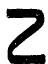
\includegraphics[keepaspectratio]{images/part002_71b18b59.jpg}}

Remarks. 1) In general, the set \(\mathcal{C}(\mathbf{X};\mathbf{Y})\) is not closed in \(\mathcal{F}(\mathbf{X};\mathbf{Y})\) with respect to the topology of pointwise convergence: in other words, a pointwise limit of continuous functions is not necessarily continuous {[}Exercise 5 a){]}.

\begin{enumerate}
\def\labelenumi{\arabic{enumi})}
\setcounter{enumi}{1}
\tightlist
\item
  A filter on \(\mathcal{C}(\mathbf{X};\mathbf{Y})\) can converge pointwise to a continuous function without converging uniformly to this function.
\end{enumerate}

For example, on the interval I = {[}0, 1{]}, let \(u_n\) be the real-valued function which is equal to 0 for \(x = 0\) and \(2/n \leqslant x \leqslant 1\) , equal to 1 for \(x = 1/n\) , and linear in each of the intervals {[}0, 1/n{]} and {[}1/n, 2/n{]}. The sequence \((u_n)\) converges pointwise to 0, but does not converge uniformly to 0 in I (cf.~Exercise 6).

\begin{enumerate}
\def\labelenumi{\arabic{enumi})}
\setcounter{enumi}{2}
\item
  If X is a uniform space, a proof analogous to that of Proposition 8 shows that the set of uniformly continuous mappings of X into Y is closed in \(\mathcal{F}_u(X;Y)\) .
\item
  Suppose that the uniform space Y carries a commutative and associative law of composition, written additively, such that the mapping \((y, y') \to y + y'\) is continuous on \(Y \times Y\) . Then, if \((u_n)\) is a sequence of continuous mappings of X into Y such that the series whose general term is \(u_n\) is uniformly convergent in X, the sum of the series is continuous on X.
\end{enumerate}

We leave it to the reader to state the corresponding result for uniformly summable families (no. 1, Remark 5) of continuous mappings.

PROPOSITION 9. Let X be a topological space, Y a uniform space. Then the mapping \((f, x) \to f(x)\) of \(\mathcal{C}_u(X; Y) \times X\) into Y is continuous.

Let \(f_0: \mathbf{X} \to \mathbf{Y}\) be a continuous mapping, let \(x_0\) be a point of \(\mathbf{X}\) and let \(\mathbf{V}\) be an entourage of \(\mathbf{Y}\) . The set \(\mathbf{T}\) of continuous mappings \(f: \mathbf{X} \to \mathbf{Y}\) such that \((f(x), f(x_0)) \in \mathbf{V}\) for all \(x \in \mathbf{X}\) is a neighbourhood of \(f_0\) in \(\mathcal{C}_u(\mathbf{X}; \mathbf{Y})\) . On the other hand, since \(f_0\) is continuous, there is a neighbourhood \(\mathbf{U}\) of \(x_0\) in \(\mathbf{X}\) such that \((f_0(x), f_0(x_0)) \in \mathbf{V}\) for all \(x \in \mathbf{U}\) . Consequently we have \((f(x), f(x_0)) \in \overset{\circ}{\mathbf{V}}\) whenever \((f, x) \in \mathbf{T} \times \mathbf{U}\) , and the result is proved.

\section{EQUICONTINUOUS SETS}

\subsection{DEFINITION AND GENERAL CRITERIA}

DEFINITION 1. Let X be a topological space and Y a uniform space. A subset H of F(X; Y) is said to be equicontinuous at a point \(x_{0} \in X\) if, for each entourage V of Y, there is a neighbourhood U of \(x_{0}\) in X such that \((f(x_{0}),f(x))\in\mathbf{V}\) for all \(x\in\mathbf{U}\) and all \(f\in\mathbf{H}\) . H is said to be equicontinuous if it is equicontinuous at every point of X.

DEFINITION 2. Let X and Y be two uniform spaces. A subset H of \(\mathcal{F}(X;Y)\) is said to be uniformly equicontinuous if, for each entourage V of Y, there exists an entourage U of X such that we have \((f(x), f(x')) \in V\) whenever \((x, x') \in U\) and \(f \in H\) .

A family \((f_{t})_{t\in I}\) of mappings of X into Y is said to be equicontinuous at a point \(x_0\) (resp. equicontinuous, uniformly equicontinuous) if the set of the \(f_{t}\) is equicontinuous at \(x_0\) (resp. equicontinuous, uniformly equicontinuous).

It is clear that if \(\mathbf{H}\subset\mathcal{F}(\mathbf{X};\mathbf{Y})\) is equicontinuous at \(x_{0}\) , then each \(f\in H\) is continuous at \(x_{0}\) ; if H is equicontinuous, then each \(f\in H\) is continuous on X, i.e.~\(\mathbf{H}\subset\mathcal{C}(\mathbf{X};\mathbf{Y})\) . Likewise, if H is uniformly equicontinuous (X being a uniform space), every \(f\in H\) is uniformly continuous on X. It is also clear that a uniformly equicontinuous set of mappings is equicontinuous; but a set of uniformly continuous mappings can be equicontinuous without being uniformly equicontinuous (see Exercise 1; Corollary 2 to Proposition 1; and no. 2, Proposition 4).

Examples. 1) Let X be a topological space (resp. a uniform space) and Y a uniform space. Every finite set of continuous (resp. uniformly continuous) mappings of X into Y is equicontinuous (resp. uniformly equicontinuous).

\begin{enumerate}
\def\labelenumi{\arabic{enumi})}
\setcounter{enumi}{1}
\tightlist
\item
  Let X, Y be two metric spaces, d (resp. d') the metric on X (resp. Y), and let k, \(\alpha\) be two real numbers \textgreater{} 0. Then the set of all mappings f: X → Y such that
\end{enumerate}

\[
d ^ {\prime} (f (x), f (x ^ {\prime})) \leqslant k (d (x, x ^ {\prime})) ^ {\alpha}
\]

for each pair of points \(x, x'\) of \(\mathbf{X}\) , is uniformly equicontinuous. For example, the set of all isometries (Chapter IX, § 2, no. 2) of \(\mathbf{X}\) onto a subset of \(\mathbf{Y}\) is uniformly equicontinuous.

* Let H be a set of real-valued functions defined on an interval I ⊂ R, which are differentiable on I and are such that \(|f'(x)| \leqslant k\) for all \(x \in I\) and all \(f \in H\) . Then H is uniformly equicontinuous, because if \(x_{1}, x_{2}\) are any two points of I we have \(|f(x_{1}) - f(x_{2})| \leqslant k |x_{1} - x_{2}|\) for each \(f \in H\) by the mean value theorem. *

\begin{enumerate}
\def\labelenumi{\arabic{enumi})}
\setcounter{enumi}{2}
\tightlist
\item
  Let G be a topological group, let Y be a uniform space and let \(f: \mathbf{G} \to \mathbf{Y}\) be a uniformly continuous mapping {[}G being endowed with its left uniformity (Chapter III, § 3, no. 1){]}. For each \(s \in \mathbf{G}\) , let \(f_s\) be the mapping \(x \to f(sx)\) of G into Y. Then the set of mappings \(f_s(s \in \mathbf{G})\) is uniformly equicontinuous, since the relation \(x^{-1}x' \in V\) is equivalent to \((sx)^{-1}(sx') \in V\) .
\end{enumerate}

PROPOSITION 1. Let T be a set, let S be a set of subsets of T, let Y be a uniform space, X a topological (resp. uniform) space, and let f be a mapping of \(\mathbf{T} \times \mathbf{X}\) into \(\mathbf{Y}\) . For each \(\mathbf{A} \in \mathfrak{S}\) , let \(\mathbf{H}_{\mathbf{A}} \subset \mathcal{F}(\mathbf{X}; \mathbf{Y})\) be the set of all mappings \(x \to f(t, x)\) as \(t\) runs through \(\mathbf{A}\) . Then the mapping \(x \to f(., x)\) of \(\mathbf{X}\) into \(\mathcal{F}_{\mathfrak{S}}(\mathbf{T}; \mathbf{Y})\) is continuous at a point \(x_0 \in \mathbf{X}\) (resp. uniformly continuous) if and only if the set \(\mathbf{H}_{\mathbf{A}}\) is equicontinuous at \(x_0\) (resp. uniformly equicontinuous) for all \(\mathbf{A} \in \mathfrak{S}\) .

Consider first the particular case where \(\mathfrak{S} = \{\mathrm{T}\}\) , i.e.~\(\mathcal{F}_{\mathfrak{S}}(\mathrm{T};\mathrm{Y}) = \mathcal{F}_u(\mathrm{T};\mathrm{Y})\) . For each entourage V of Y, the condition \((f(.,x),f(.,x'))\in W(\mathrm{V})\) signifies that \((f(t,x),f(t,x'))\in \mathrm{V}\) for all \(t\in \mathrm{T}\) . To say that \(x\to f(.,x)\) is continuous at \(x_0\) (resp. is uniformly continuous) is therefore equivalent to saying that, for each entourage V of Y, there is a neighbourhood U of \(x_0\) in X (resp. an entourage M of X) such that the relation \(x\in \mathrm{U}\) {[}resp. \((x,x')\in \mathrm{M}]\) implies \((f(t,x),f(t,x_0))\in \mathrm{V}\) {[}resp. \((f(t,x),f(t,x'))\in \mathrm{V}]\) for all \(t\in \mathrm{T}\) , and the proposition follows from Definitions 1 and 2. In the general case, we have to express that, for each \(\mathrm{A}\in \mathfrak{S}\) , the mapping \(x\rightarrow f(.,x)|\mathrm{A}\) of X into \(\mathcal{F}_u(\mathrm{A};\mathrm{Y})\) is continuous at \(x_0\) (resp. uniformly continuous), by virtue of § 1, no. 2; from what has been said, this is equivalent to saying that, for each \(\mathrm{A}\in \mathfrak{S}\) , \(\mathrm{H}_{\mathrm{A}}\) is equicontinuous at \(x_0\) (resp. uniformly equicontinuous).

Proposition 1 allows us to translate Definitions 1 and 2 into forms which are sometimes useful, by applying it to the case where \(\mathbf{T} = \mathbf{H}\) and \(f\) is the mapping \((h, x) \to h(x)\) of \(\mathbf{H} \times \mathbf{X}\) into \(\mathbf{Y}\) ; since \(f(., x)\) is the mapping \(h \to h(x)\) of \(\mathbf{H}\) into \(\mathbf{Y}\) , we see that:

COROLLARY 1. Let X be a topological (resp. uniform) space, Y a uniform space and H a subset of \(\mathcal{F}\) (X; Y). For each \(x \in \mathbf{X}\) , let \(\tilde{x}\) denote the mapping \(h \to h(x)\) of H into Y. Then H is equicontinuous at \(x_0\) (resp. uniformly equicontinuous) if and only if the mapping \(x \to \tilde{x}\) of X into the uniform space \(\mathcal{F}_u\) (H; Y) is continuous at \(x_0\) (resp. uniformly continuous).

In particular, if X is compact, every continuous mapping of X into \(\mathcal{F}_{u}(H;Y)\) is uniformly continuous (Chapter II, § 4, no. 1, Theorem 2). Therefore:

COROLLARY 2. Let X be a compact space, Y a uniform space. Then every equicontinuous subset of \(\mathcal{F}(X;Y)\) is uniformly equicontinuous.

Now suppose we have a set T, a topological space X, a uniform space Y and a mapping \(f: T \times X \to Y\) . Let \(\tilde{f}\) denote the mapping \(x \to f(., x)\) of X into \(\mathcal{F}_{u}(T; Y)\) , and let us consider the canonical mapping \(\theta: (t, g) \to g(t)\) of \(T \times \mathcal{F}_{u}(T; Y)\) into Y. It is clear that the diagram

\[
\mathrm{T} \times \mathrm{X} \xrightarrow {f} \mathrm{Y}
\]

\[
\iota_ {\mathrm{T}} \times \tilde {f} \searrow \nearrow \theta
\]

\[
\mathbf {T} \times \mathcal {F} _ {u} (\mathbf {T}; \mathbf {Y})
\]

(where \(\iota_{\mathbf{T}}\) is the identity mapping of T) is commutative. Suppose now that T is endowed with a topology and that, for each \(x \in \mathbf{X}\) , the mapping \(f(., x): t \to f(t, x)\) is continuous; we can then replace \(\mathcal{F}_{u}(\mathrm{T}; \mathrm{Y})\) by \(\mathcal{C}_{u}(\mathrm{T}; \mathrm{Y})\) in the above diagram. But we know that \(\theta\) is continuous from § 1, no. 6, Proposition 9; hence if \(\tilde{f}\) is continuous it follows that \(f\) is continuous. Since the continuity of \(\tilde{f}\) can be expressed with the help of Proposition 1, we obtain the following result:

COROLLARY 3. Let T, X be topological spaces, let Y be a uniform space and let f be a mapping of T × X into Y. Then f is continuous, provided that the following conditions are satisfied:

\begin{enumerate}
\def\labelenumi{\arabic{enumi})}
\item
  For each \(x \in \mathbf{X}\) , the partial mapping \(t \to f(t, x)\) is continuous.
\item
  As \(t\) runs through \(\mathbf{T}\) , the partial mappings \(x \to f(t, x)\) form an equicontinuous subset of \(\mathfrak{F}(\mathbf{X}; \mathbf{Y})\) .
\end{enumerate}

In particular, take T to be a subset H of \(\mathcal{F}(\mathbf{X};\mathbf{Y})\) and \(f\) to be the canonical mapping \((h,x)\to h(x)\) of \(\mathbf{H}\times \mathbf{X}\) into Y; condition 1) of Corollary 3 means that H is endowed with a topology finer than that of pointwise convergence, and condition 2) means that H is equicontinuous. Hence:

COROLLARY 4. Let X be a topological space, Y a uniform space, H an equicontinuous set of mappings of X into Y. If H is endowed with the topology of pointwise convergence, then the mapping \((h, x) \to h(x)\) of \(H \times X\) into Y is continuous.

More intuitively, this expresses the fact that if \(h \in \mathbf{H}\) converges pointwise to \(h_0 \in \mathbf{H}\) and if \(x \in \mathbf{X}\) converges to \(x_0\) , then \(h(x)\) converges to \(h_0(x_0)\) .

COROLLARY 5. Let X be a topological space, let Y, Z be two uniform spaces and let H be an equicontinuous set of mappings of Y into Z. If H, C(X; Y) and C(X; Z) are endowed with the topology of pointwise convergence, then the mapping \((u, v) \to u \circ v\) of H × C(X; Y) into C(X; Z) is continuous.

We have to show that, for each \(x \in \mathbf{X}\) , the mapping \((u, v) \to u(v(x))\) of \(\mathbf{H} \times \mathcal{C}(\mathbf{X}; \mathbf{Y})\) into \(\mathbf{Z}\) is continuous. Now \(v \to v(x)\) is continuous on \(\mathbf{H}\) ( \(\S 1\) , no. 2, Remark 6), and it follows from Corollary 4 that \((u, y) \to u(y)\) is a continuous mapping of \(\mathbf{H} \times \mathbf{Y}\) into \(\mathbf{Z}\) ; since \((u, v) \to u(v(x))\) is the composition of \((u, y) \to u(y)\) and \((u, v) \to (u, v(x))\) , the result is proved.

The following proposition and its corollary are the analogues of Corollaries 3 and 4 of Proposition 1 for uniformly equicontinuous sets of mappings:

PROPOSITION 2. Let T, X, Y be uniform spaces and let f be a mapping of T × X into Y. Then f is uniformly continuous if and only if the following two conditions are satisfied:

\begin{enumerate}
\def\labelenumi{\arabic{enumi})}
\item
  The mappings \(x \to f(t, x)\) ( \(t \in \mathbf{T}\) ) form a uniformly equicontinuous subset of \(\mathcal{F}(\mathbf{X}; \mathbf{Y})\) .
\item
  The mappings \(t \to f(t, x)\) ( \(x \in \mathbf{X}\) ) form a uniformly equicontinuous subset of \(\mathcal{F}(\mathbf{T}; \mathbf{Y})\) .
\end{enumerate}

It is easily seen that the conditions are necessary. Conversely, suppose that they are satisfied. Let W be an entourage of Y; then there exists an entourage U of T and an entourage V of X such that: 1) \((t', t'') \in \mathbf{U}\) implies that, for each \(x \in X\) ,

\[
\left(f \left(t ^ {\prime}, x\right), f \left(t ^ {\prime \prime}, x\right)\right) \in W.
\]

\begin{enumerate}
\def\labelenumi{\arabic{enumi})}
\setcounter{enumi}{1}
\tightlist
\item
  \((x', x'') \in \mathbf{V}\) implies that, for each \(t \in \mathbf{T}\) ,
\end{enumerate}

\[
(f (t, x ^ {\prime}), f (t, x ^ {\prime \prime})) \in W.
\]

It is now clear that the relation `` \((t', t'') \in \mathbf{U}\) and \((x', x'') \in \mathbf{V}\) '' implies that \((f(t', x'), f(t'', x'')) \in \overset{2}{\mathbf{W}}\) , whence the result.

In particular, take T to be a subset H of \(\mathcal{F}(\mathbf{X};\mathbf{Y})\) , endowed with the uniformity of uniform convergence, and take \(f\) to be the canonical mapping \((h,x)\to h(x)\) ; then condition 2) of Proposition 2 is automatically satisfied because, for each entourage W of Y, the set of pairs \((h',h'')\) such that \((h'(x),h''(x))\in W\) for all \(x\in X\) is by definition an entourage of the uniform structure of H. Hence only condition 1) has to be expressed; in other words:

COROLLARY. Let X, Y be two uniform spaces and let H be a subset of \(\mathcal{F}(X;Y)\) . Then H is uniformly equicontinuous if and only if the mapping \((h,x) \to h(x)\) of \(H \times X\) into Y is uniformly continuous, H being endowed with the uniformity of uniform convergence.

\subsection{SPECIAL CRITERIA FOR EQUICONTINUITY}

It is clear that every subset of an equicontinuous (resp. uniformly equicontinuous) set is equicontinuous (resp. uniformly equicontinuous). Again, if X is a topological (resp. uniform) space and Y is a uniform space, every finite union of equicontinuous (resp. uniformly equicontinuous) subsets of \(\mathcal{F}(X;Y)\) is equicontinuous (resp. uniformly equicontinuous).

Let \(X, X'\) be two topological (resp. uniform) spaces, let \(Y, Y'\) be two uniform spaces, let \(f: X \to X'\) be a continuous (resp. uniformly continuous) mapping and let \(g: Y \to Y'\) be a uniformly continuous mapping.

It follows immediately from the definitions that the mapping \(u \rightarrow g \circ u \circ f\) of \(\mathcal{F}(X; Y)\) into \(\mathcal{F}(X'; Y')\) transforms equicontinuous (resp. uniformly equicontinuous) sets into equicontinuous (resp. uniformly equicontinuous) sets.

PROPOSITION 3. Let X be a topological (resp. uniform) space, let \((\mathbf{Y}_{t})_{t \in I}\) be a family of uniform spaces, let Y be a set, and for each \(t \in I\) , let \(f_{t}\) be a mapping of Y into \(\mathbf{Y}_{t}\) . Let Y be endowed with the coarsest uniformity for which all the \(f_{t}\) are uniformly continuous. For a subset H of \(\mathcal{F}(\mathbf{X}; \mathbf{Y})\) to be equicontinuous (resp. uniformly equicontinuous) it is necessary and sufficient that, for each \(t \in I\) , the image of H under the mapping \(u \to f_{t} \circ u\) be an equicontinuous (resp. uniformly equicontinuous) subset of \(\mathcal{F}(\mathbf{X}; \mathbf{Y}_{t})\) .

This is an immediate consequence of Definitions 1 and 2 and the definition of the entourages of Y.

PROPOSITION 4. Let X, Y be two uniform spaces and let H be a set of uniformly continuous mappings of X into Y. Let \(\hat{X}, \hat{Y}\) be the Hausdorff completions of X, Y respectively, and let \(\tilde{H}\) denote the set of mappings \(\hat{u}: \hat{X} \to \hat{Y}\) as \(u\) runs through H (Chapter II, § 3, no. 7, Proposition 15). Then H is uniformly equicontinuous if and only if \(\tilde{H}\) is uniformly equicontinuous.

We recall that the diagram

\[
\begin{array}{c} \mathbf {X} \xrightarrow {u} \mathbf {Y} \\ i \downarrow \quad \quad \quad \quad \quad \quad \quad \quad \quad \quad \quad \quad \quad j \\ \hat {\mathbf {X}} \xrightarrow {\hat {u}} \hat {\mathbf {Y}} \end{array}\tag{1}
\]

is commutative, where \(i\) and \(j\) are the canonical mappings; moreover, the uniformity of \(\mathbf{X}\) (resp. \(\mathbf{Y}\) ) is the inverse image under \(i\) (resp. \(j\) ) of that of \(\hat{\mathbf{X}}\) (resp. \(\hat{\mathbf{Y}}\) ). Hence \(\mathbf{H}\) is uniformly equicontinuous if and only if its image under the mapping \(u \to j \circ u\) is uniformly equicontinuous (Proposition 3), and we may already restrict ourselves to the case where \(\mathbf{Y}\) is Hausdorff and complete; moreover, if \(\tilde{\mathbf{H}}\) is uniformly equicontinuous then so is \(\mathbf{H}\) , because it is the image of \(\tilde{\mathbf{H}}\) under the mapping \(\hat{u} \to \hat{u} \circ i\) ; thus it remains to prove the converse when \(\mathbf{Y} = \hat{\mathbf{Y}}\) . Let \(\mathbf{V}\) be a closed entourage of \(\mathbf{Y}\) ; by hypothesis there is an entourage \(\mathbf{U}\) of \(\mathbf{X}\) such that the relations \((x, x') \in \mathbf{U}\) and \(u \in \mathbf{H}\) imply that \((u(x), u(x')) \in \mathbf{V}\) . Now, if \(\mathbf{U}'\) is the image of \(\mathbf{U}\) under \(i \times i\) , the closure \(\overline{\mathbf{U}'}\) of \(\mathbf{U}'\) in \(\hat{\mathbf{X}} \times \hat{\mathbf{X}}\) is an entourage of \(\hat{\mathbf{X}}\) (Chapter II, § 3, no. 7, Proposition 12); the hypothesis implies that, whenever \((z, z') \in \mathbf{U}'\) and \(u \in \mathbf{H}\) , we have \((\hat{u}(z), \hat{u}(z')) \in \mathbf{V}\) . Since \(\mathbf{V}\) is closed and \(\hat{u}\) is continuous, we have also \((\hat{u}(t), \hat{u}(t')) \in \mathbf{V}\) for all \((t, t') \in \overline{\mathbf{U}'}\) and all \(u \in \mathbf{H}\) ; this completes the proof.

PROPOSITION 5. Let G, G' be two topological groups endowed with their left uniformities, and let H be a set of homomorphisms of G into G'. Then the following conditions are equivalent:

\begin{enumerate}
\def\labelenumi{\alph{enumi})}
\item
  H is equicontinuous at the identity element e of G,
\item
  H is equicontinuous,
\item
  H is uniformly equicontinuous.
\end{enumerate}

It is enough to show that a) implies c). Let \(V'\) be a neighbourhood of the identity element \(e'\) of \(G'\) ; then, by hypothesis, there is a neighbourhood V of e in G such that \(u(V) \subset V'\) for all \(u \in H\) ; since the elements of H are homomorphisms, the relation \(x^{-1}y \in V\) implies that we have

\[
(u (x)) ^ {- 1} u (y) = u (x ^ {- 1} y) \in \mathbf {V} ^ {\prime}.
\]

In view of the definition of the entourages of the left uniformities of G and G' (Chapter III, § 3, no. 1), the result follows.

\subsection{CLOSURE OF AN EQUICONTINUOUS SET}

PROPOSITION 6. Let X be a topological (resp. uniform) space, let Y be a uniform space and let H be a subset of \(\mathcal{F}(X;Y)\) . Then H is equicontinuous at a point \(x_0 \in X\) (resp. uniformly equicontinuous) if and only if the closure \(\overline{\mathbf{H}}\) of H in \(\mathcal{F}_s(X;Y)\) is equicontinuous at \(x_0\) (resp. uniformly equicontinuous).

The condition is sufficient, trivially. To show that it is necessary, consider an entourage V of Y which is closed in \(Y \times Y\) ; by hypothesis, there is a neighbourhood U of \(x_{0}\) in X (resp. an entourage M of X) such that the relation \(x \in U\) (resp. \((x', x'') \in M\) ) implies \((h(x_{0}), h(x)) \in V\) {[}resp. \((h(x'), h(x'')) \in V\) {]} for all \(h \in H\) . Since V is closed, the mappings \(h \in \mathcal{F}(X; Y)\) which satisfy the relation \((h(x_{0}), h(x)) \in V\) for all \(x \in U\) {[}resp. the relation \((h(x'), h(x'')) \in V\) for all \((x', x'') \in M\) {]} form a closed subset of \(\mathcal{F}_{s}(X; Y)\) (§ 1, no. 2, Remark 6); since this closed subset contains H, it contains \(\overline{H}\) . Hence the result, since the closed entourages of Y form a fundamental system of entourages (Chapter II, § 1, no. 2, Proposition 2, Corollary 2).

\subsection{POINTWISE CONVERGENCE AND COMPACT CONVERGENCE ON EQUICONTINUOUS SETS}

THEOREM 1. Let X be a topological (resp. uniform) space, let Y be a uniform space and let H be an equicontinuous (resp. uniformly equicontinuous) subset of C(X;Y). Then the following uniformities on H are identical: the uniformity of compact (resp. precompact) convergence, the uniformity of pointwise convergence and the uniformity of pointwise convergence in a dense subset D of X.

It is enough to show that the last uniformity on H is finer than the first; in other words that, given an entourage V of Y and a compact (resp. precompact) subset A of X, there exists an entourage W of Y and a finite subset F of D such that the relation

\[
u \in \mathrm{H}, \quad v \in \mathrm{H} \quad \text { and } \quad (u (x), v (x)) \in \mathrm{W} \quad \text { for   all } \quad x \in \mathrm{F}\tag{2}
\]

implies

\[
(u (x), v (x)) \in \mathbf {V} \quad \text { for   all } \quad x \in \mathbf {A}.\tag{3}
\]

Suppose first that A is compact and H equicontinuous. Given a symmetric entourage W of Y, every point \(x \in X\) has a neighbourhood \(\mathrm{U}(x)\) such that the relation \(x' \in \mathrm{U}(x)\) implies \((u(x), u(x')) \in \mathrm{W}\) for all \(u \in H\) . We can therefore cover the compact set A by a finite number of open sets \(U_i\) such that, for each pair of points \(x', x''\) of the same set \(U_i\) , we have \((u(x'), u(x'')) \in \dot{\mathbf{W}}\) for all \(u \in H\) . Let \(a_i\) be a point of \(D \cap U_i\) , let F be the set of the \(a_i\) , and suppose that (2) is true; then for each \(x \in A\) there exists an index i such that \(a_i\) and x belong to the same set \(U_i\) , so that we have \((u(x), u(a_i)) \in \dot{\mathbf{W}}\) and \((v(a_i), v(x)) \in \dot{\mathbf{W}}\) ; thus (2) implies (3) provided that W is chosen so that \(W \subset V\) .

If A is precompact and H uniformly equicontinuous, we use Proposition 4 of no. 2; it is enough to note that \(i(\overline{\mathbf{A}})\) is compact in \(\hat{\mathbf{X}}\) , \(i(\mathbf{D})\) dense in \(\hat{\mathbf{X}}\) and that the entourages of Y are the inverse images of those of \(\hat{Y}\) under the mapping \(j \times j\) .

COROLLARY. Under the hypotheses of Theorem 1, the closure \(\overline{\mathbf{H}}\) of \(\mathbf{H}\) in \(\mathcal{F}(\mathbf{X};\mathbf{Y})\) with respect to the topology of pointwise convergence is the same as the closure of \(\mathbf{H}\) in \(\mathcal{C}(\mathbf{X};\mathbf{Y})\) with respect to the topology of compact (resp. precompact) convergence.

For the set \(\overline{H}\) is equicontinuous (resp. uniformly equicontinuous) by Proposition 6 of no. 3, and hence is contained in C(X; Y); the result follows immediately from the fact that, on \(\overline{H}\) , the two topologies under consideration are the same, by virtue of Theorem 1.

\subsection{COMPACT SETS OF CONTINUOUS MAPPINGS}

THEOREM 2 (Ascoli). Let X be a topological (resp. uniform) space, let S be a covering of X, let Y be a uniform space and H a set of mappings of X into Y such that, for each A ∈ S and each u ∈ H, the restriction of u to A is continuous (resp. uniformly continuous). Then, for H to be precompact with respect to the uniformity of S-convergence, it is necessary in all cases and also sufficient if the sets \(\mathbf{A} \in \mathfrak{S}\) are compact (resp. precompact) that the following conditions should be satisfied:

\begin{enumerate}
\def\labelenumi{\alph{enumi})}
\item
  For each \(\mathbf{A} \in \mathfrak{S}\) , the set \(\mathbf{H}|\mathbf{A} \subset \mathcal{F}(\mathbf{A};\mathbf{Y})\) of restrictions to \(\mathbf{A}\) of functions of \(\mathbf{H}\) is equicontinuous (resp. uniformly equicontinuous).
\item
  For each \(x \in \mathbf{X}\) , the set \(\mathbf{H}(x) \subset \mathbf{Y}\) of points \(u(x)\) ( \(u \in \mathbf{H}\) ) is precompact.
\end{enumerate}

\begin{enumerate}
\def\labelenumi{\arabic{enumi})}
\tightlist
\item
  Let us show first that conditions a) and b) are necessary. We know (§ 1, no. 2, Remark 6) that the mapping \(u \to u(x)\) of \(\mathcal{F}_{\mathfrak{S}}(\mathbf{X};\mathbf{Y})\) into Y is uniformly continuous; hence, if H is precompact, so is \(\mathbf{H}(x)\) (Chapter II, § 4, no. 2, Proposition 2), which proves b). To prove a), consider a set \(\mathbf{A} \in \mathfrak{S}\) , a point \(x_0 \in \mathbf{A}\) and an entourage V of Y; since H is precompact it can be covered by a finite number of \(W(\mathbf{A},\mathbf{V})\) -small sets; in other words there is a finite sequence \((u_i)\) of elements of H such that, for each \(u \in \mathbf{H}\) , we have
\end{enumerate}

\[
(u (x), u _ {i} (x)) \in \mathbf {V} \quad \text { for   all } \quad x \in \mathbf {A}\tag{4}
\]

for at least one index i.

Since each of the \(u_{i}|A\) is continuous at \(x_{0}\) (resp. uniformly continuous) there is a neighbourhood \(U_{i}\) of \(x_{0}\) in A (resp. an entourage \(M_{i}\) of A) such that

\[
x \in \mathrm{U} _ {i} \quad \text { implies } \quad (u _ {i} (x), u _ {i} (x _ {0})) \in \mathrm{V},\tag{5}
\]

(resp. such that

\[
(x ^ {\prime}, x ^ {\prime \prime}) \in \mathbf {M} _ {i} \quad \text { implies } \quad (u _ {i} (x ^ {\prime}), u _ {i} (x ^ {\prime \prime})) \in \mathbf {V}.\tag{6}
\]

Let U (resp. M) be the intersection of the \(U_{i}\) (resp. \(M_{i}\) ); it is a neighbourhood of \(x_{0}\) in A (resp. an entourage of A). For each \(u \in H\) there is an index i for which (4) holds; writing condition (4) for \(x_{0}\) and for x (resp. for \(x'\) and \(x''\) ) and taking account of (5) {[}resp. (6){]}, we see immediately that the relation \(x \in U\) {[}resp. \((x', x'') \in M\) {]} implies \((u(x), u(x_{0})) \in \overset{\mathbf{3}}{\mathrm{V}}\) {[}resp. \((u(x'), u(x'')) \in \overset{\mathbf{3}}{\mathrm{V}}\) {]}, for each \(u \in H\) ; and this establishes a).

\begin{enumerate}
\def\labelenumi{\arabic{enumi})}
\setcounter{enumi}{1}
\tightlist
\item
  Now let us show that the conditions a) and b) are sufficient if the sets \(A \in S\) are compact (resp. precompact). Condition b) implies that H is precompact with respect to the uniformity of pointwise convergence (Chapter II, § 4, no. 2, Proposition 3). But it follows from condition a) and Theorem 1 of no. 4 that on H\textbar A the uniformity of pointwise convergence in A coincides with the uniformity of uniform convergence in A; hence H\textbar A is precompact in \(\mathcal{F}_{u}(A; Y)\) , which implies that H is precompact with respect to the uniformity of S-convergence (§ 1, no. 2).
\end{enumerate}

Note that condition b) of Theorem 2 is automatically satisfied if Y is a precompact space.

COROLLARY 1. Let X be a topological (resp. uniform) space, let Y be a Hausdorff uniform space and let H be an equicontinuous (resp. uniformly equicontinuous) subset of \(\mathcal{C}(\mathbf{X};\mathbf{Y})\) . Suppose that \(\mathrm{H}(x)\) is relatively compact in Y for each \(x\in \mathbf{X}\) . Then H is relatively compact in \(\mathcal{C}(\mathbf{X};\mathbf{Y})\) with respect to the topology of compact (resp. precompact) convergence.

Let \(\overline{\mathbf{H}}\) be the closure of \(\mathbf{H}\) in \(\mathcal{F}_s(\mathbf{X};\mathbf{Y})\) . \(\overline{\mathbf{H}}\) is equicontinuous (resp. uniformly equicontinuous) (no. 3, Proposition 6). Moreover, we have \(\overline{\mathbf{H}}(x)\subset \overline{\mathbf{H}(x)}\) ( \(\S\) 1, no. 2, Remark 6) and therefore \(\overline{\mathbf{H}}(x)\) is also relatively compact; hence Theorem 2 shows that \(\overline{\mathbf{H}}\) is precompact with respect to \(\mathfrak{S}\) -convergence, where \(\mathfrak{S}\) denotes the set of all compact (resp. precompact) subsets of \(\mathbf{X}\) . Moreover, since \(\overline{\mathbf{H}(x)}\) is compact, and therefore complete, \(\overline{\mathbf{H}}\) is complete with respect to the uniformity of pointwise convergence (Chapter II, \(\S\) 3, no. 5, Proposition 10 and no. 4, Proposition 8) and therefore also with respect to the uniformity of \(\mathfrak{S}\) -convergence ( \(\S\) 1, no. 5, Proposition 5, Corollary 2); \(\overline{\mathbf{H}}\) is therefore compact, since it is precompact, complete and Hausdorff ( \(\S\) 1, no. 2, Proposition 1).

COROLLARY 2. Let X be a topological (resp. uniform) space, let Y be a complete Hausdorff uniform space and let H be an equicontinuous (resp. uniformly equicontinuous) subset of C(X; Y). Suppose that H(x) is relatively compact in Y for all \(x \in D\) , where D is a dense subset of X. Then H is relatively compact in C(X; Y) with respect to the topology of compact (resp. precompact) convergence.

It is enough to show that \(\mathrm{H}(x)\) is relatively compact for all \(x \in X\) , for we can then apply Corollary I. Since Y is complete it is enough to show that \(\mathrm{H}(x)\) is precompact for all \(x \in X\) . Now if V is any symmetric entourage of Y, there is a neighbourhood U of x such that \((u(x), u(x')) \in V\) for all \(x' \in U\) and all \(u \in H\) . By hypothesis there exists \(x' \in U \cap D\) , and since \(\mathrm{H}(x')\) is relatively compact in Y, there exists a finite number of points \(y_k \in Y\) such that \(\mathrm{H}(x')\) is contained in the union of the sets \(\mathrm{V}(y_k)\) ; hence \(\mathrm{H}(x)\) is contained in the union of the sets \(\overset{2}{\mathrm{V}}(y_k)\) , and the proof is complete.

COROLLARY 3. Let X be a locally compact space, Y a Hausdorff uniform space, H a subset of C (X; Y). Then H is relatively compact in \(\mathcal{C}_c(X; Y)\) if and only if H is equicontinuous and H(x) relatively compact in Y for all \(x \in \mathbf{X}\) .

In view of Corollary 1 it is enough to show that, if H is relatively compact in \(\mathcal{C}_{c}(\mathbf{X};\mathbf{Y})\) , then H is equicontinuous. Now each point \(x\in X\) has a compact neighbourhood A, and it follows from Theorem 2 that H/A is equicontinuous; this implies that H is equicontinuous at x, and the result is proved.

Remark. Let X be a topological space, Y a uniform space and S a set of subsets of X. Then on every precompact subset H of \(\mathcal{F}_{\mathfrak{S}}(X;Y)\) , the uniformity of S-convergence is the same as the uniformity of pointwise convergence in \(B = \bigcup_{A \in \mathfrak{S}} A\) . We can reduce to the case where \(B = X\) and Y is Hausdorff and complete; for if \(j\) is the canonical injection \(B \to X\) and \(i\) the canonical mapping \(Y \to \hat{Y}\) , the uniformity of S-convergence on \(\mathcal{F}(X;Y)\) is the inverse image of the uniformity of S-convergence on \(\mathcal{F}(B;\hat{Y})\) under the mapping \(\theta : u \to i \circ u \circ j\) ( \(\S 1\) , no. 4, Proposition 4), and H is precompact if and only if \(\theta(H)\) is (Chapter II, \(\S 4\) , no. 2, Proposition 3). This being so, if \(B = X\) and Y is Hausdorff and complete, \(\mathcal{F}_{\mathfrak{S}}(X;Y)\) is Hausdorff and complete ( \(\S 1\) , no. 2, Proposition 1 and no. 5, Theorem 1); hence the closure \(\overline{H}\) of H in this space is compact. On \(\overline{H}\) , the topology of pointwise convergence is Hausdorff ( \(\S 1\) , no. 2, Proposition 1) and coarser than that of S-convergence; hence these two topologies coincide (Chapter I, \(\S 9\) , no. 4, Theorem 2, Corollary 3) and consequently so do the uniformities of S-convergence and pointwise convergence (Chapter II, \(\S 4\) , no. 1, Theorem 1).

\section{SPECIAL FUNCTION SPACES}

\subsection{SPACES OF MAPPINGS INTO A METRIC SPACE}

Let X be a set, Y a uniform space, \((f_{t})_{t\in I}\) a family of pseudometrics defining the uniform structure of Y (Chapter IX, § 1, no. 4), and let S be a set of subsets of X. For each \(t\in I\) , each set \(A\in S\) , and each pair \((u,v)\) of mappings of X into Y, write

\[
g _ {t, \mathrm{A}} (u, v) = \sup _ {x \in \mathrm{A}} f _ {t} (u (x), v (x));
\]

it follows immediately that \(g_{t,\mathbf{A}}\) is a pseudometric on \(\mathcal{F}(\mathbf{X};\mathbf{Y})\) and that the family of pseudometrics \((g_{t,\mathbf{A}})_{t\in \mathbf{I},\mathbf{A}\in \mathfrak{S}}\) defines the uniformity of \(\mathfrak{S}\) -convergence on \(\mathcal{F}(\mathbf{X};\mathbf{Y})\) . In particular:

PROPOSITION I. If Y is a metrizable uniform space, the uniformity of uniform convergence on \(\mathcal{F}(X;Y)\) is metrizable.

For if d is a metric on Y compatible with its uniform structure, the structure of uniform convergence on \(\mathcal{F}(X;Y)\) is defined by the single pseudometric

\[
\delta (u, v) = \sup _ {x \in \mathbf {X}} d (u (x), v (x));
\]

in general this pseudometric is not finite, but it is equivalent to a finite one (Chapter IX, § 1, no. 2), and since the uniformity of uniform convergence is Hausdorff (§ 1, no. 2, Proposition 1), it is metrizable.

COROLLARY. Let X be a topological space and let Y be a metrizable uniform space. Suppose that there is a sequence \((\mathbf{K}_{n})\) of compact subsets of X such that every compact subset of X is contained in some \(K_{n}\) . Then the uniformity of compact convergence on \(\mathcal{F}(\mathbf{X};\mathbf{Y})\) is metrizable.

Since the \(\mathbf{K}_n\) cover \(\mathbf{X}\) , \(\mathcal{F}_c(\mathbf{X};\mathbf{Y})\) is isomorphic to a uniform subspace of \(\prod_{n}\mathcal{F}_{u}(\mathbf{K}_{n};\mathbf{Y})\) ( \(\S 1\) , no. 2, Remark 3), and the corollary therefore

follows from Proposition 1 (Chapter IX, § 2, no. 4, Theorem 1, Corollary 2).

Note that this corollary applies in particular if X is locally compact and σ-compact (Chapter I, § 9, no. 9, Proposition 15, Corollary 1).

Now let Y be a metric space and let d be its metric. If X is any set and S any set of subsets of X, we shall denote by \(\mathcal{B}_{\mathfrak{S}}(X;Y)\) the set of all mappings \(u:X\to Y\) such that \(u(A)\) is bounded for each \(A\in S\) . Unless the contrary is expressly stated we shall regard \(\mathcal{B}_{\mathfrak{S}}(X;Y)\) as endowed with the uniformity of S-convergence, which is defined by the following family of pseudometrics on \(\mathcal{B}_{\mathfrak{S}}(X;Y)\) :

\[
d _ {\mathbf {A}} (u, v) = \sup _ {x \in \mathbf {A}} d (u (x), v (x))\tag{A ∈ S}
\]

which are finite by hypothesis. When \(\mathfrak{S} = \{\mathbf{X}\}\) , we write \(\mathcal{B}(\mathbf{X};\mathbf{Y})\) in place of \(\mathcal{B}_{\mathfrak{S}}(\mathbf{X};\mathbf{Y})\) . A mapping \(u:\mathbf{X}\to \mathbf{Y}\) is said to be bounded if it belongs to \(\mathcal{B}(\mathbf{X};\mathbf{Y})\) , i.e.~if \(u(\mathbf{X})\) is a bounded subset of \(\mathbf{Y}\) .

PROPOSITION 2. Let X be a set and Y a metric space. The set \(\mathcal{B}(X;Y)\) of bounded mappings is both open and closed in the space \(\mathcal{F}_{u}(X;Y)\) .

If \(u\) is bounded, then every mapping \(v: \mathbf{X} \to \mathbf{Y}\) such that for all \(x \in \mathbf{X}\) , we have \(d(u(x), v(x)) \leqslant 1\) is bounded, because

\[
d (v (x), v (x _ {0})) \leqslant d (u (x), u (x _ {0})) + 2;
\]

hence \(\mathcal{B}(\mathbf{X};\mathbf{Y})\) is open. On the other hand, if \(u\) lies in the closure of \(\mathcal{B}(\mathbf{X};\mathbf{Y})\) in \(\mathcal{F}_u(\mathbf{X};\mathbf{Y})\) , there is a mapping \(u_0\in \mathcal{B}(\mathbf{X};\mathbf{Y})\) such that \(d(u(x),u_0(x))\leqslant 1\) for all \(x\in \mathbf{X}\) ; hence \(u\) is bounded.

COROLLARY I. Let X be a set and Y a metric space. Then \(\mathcal{B}_{\mathfrak{S}}(X;Y)\) is closed in \(\mathcal{F}_{\mathfrak{S}}(X;Y)\) . In particular, if Y is complete then \(\mathcal{B}_{\mathfrak{S}}(X;Y)\) is complete with respect to the uniformity of \(\mathfrak{S}\) -convergence.

For \(\mathcal{B}_{\mathfrak{S}}(\mathbf{X};\mathbf{Y})\) is the inverse image of the subset \(\prod_{\mathbf{A}\in \mathfrak{S}}\mathcal{B}(\mathbf{A};\mathbf{Y})\) of the product \(\prod_{\mathbf{A}\in \mathfrak{S}}\mathcal{F}_u(\mathbf{X};\mathbf{Y})\) under the canonical mapping of \(\mathcal{F}_{\mathfrak{S}}(\mathbf{X};\mathbf{Y})\) into \(\prod_{\mathbf{A}\in \mathfrak{S}}\mathcal{F}_u(\mathbf{A};\mathbf{Y})\) ; the first assertion therefore follows from § 1, no. 2, Remark 3, and the second follows from the first, if we take account of Theorem 1 of § 1, no. 5.

COROLLARY 2. Let X be a topological space and Y a metric space. Then the space of all bounded continuous mappings of X into Y is both open and closed in \(\mathcal{C}_u(X;Y)\) ; it is complete if Y is complete.

The space in question is \(\mathcal{B}(\mathbf{X};\mathbf{Y})\cap \mathcal{C}_u(\mathbf{X};\mathbf{Y})\) ; the first assertion follows from Proposition 2; the second follows from the first (§ 1, no. 6, Theorem 2, Corollary 1).

\subsection{SPACES OF MAPPINGS INTO A NORMED SPACE}

Consider, more particularly, the situation in which Y is a normed vector space over a non-discrete valued division ring K (Chapter IX, § 3, no. 3). Let us denote by \(||y||\) the norm of \(y \in Y\) . The set \(\mathcal{F}(X;Y) = Y^{\mathbf{X}}\) is then canonically endowed with a K-vector space structure. A mapping \(u: X \to Y\) is bounded if and only if the real-valued function \(x \to ||u(x)||\) is bounded in X. If \(u, v\) are bounded mappings of X into Y, it is clear that \(u + v\) and \(\lambda u (\lambda \in K)\) are bounded; in other words, \(\mathcal{B}(X;Y)\) is a vector subspace of \(\mathcal{F}(X;Y)\) . Moreover, \(||u|| = \sup_{x \in X} ||u(x)||\) is a norm on \(\mathcal{B}(X;Y)\) ; for it satisfies the triangle inequality and \(||u|| = 0\) implies \(u = 0\) , and for each \(\lambda \in K\) we have

\[
| | \lambda u | | = \sup _ {x \in \mathbf {X}} | | \lambda u (x) | | = \sup _ {x \in \mathbf {X}} | \lambda |. | | u (x) | | = | \lambda |. \sup _ {x \in \mathbf {X}} | | u (x) | | = | \lambda |. | | u | |.
\]

Moreover, it is immediately verified that the uniformity on \(\mathcal{B}(\mathbf{X};\mathbf{Y})\) defined by this norm is the uniformity of uniform convergence. Unless the contrary is expressly stated, whenever \(\mathcal{B}(\mathbf{X};\mathbf{Y})\) is considered as a normed space, it is the norm defined above which is in question.

PROPOSITION 3. If the normed space Y is complete, then every series \((u_n)\) of bounded mappings of X into Y which is absolutely convergent in the normed space \(\mathcal{B}\) (X; Y) (i.e.~which is such that \(\sum_{n=0}^{\infty}||u_n|| < +\infty\) ; cf.~Chapter IX, § 3, no. 6) is uniformly convergent in X.

For since \(\mathcal{B}(\mathbf{X};\mathbf{Y})\) is complete (no. 1, Proposition 2, Corollary 1), the result follows from Chapter IX, § 3, no. 6, Proposition 11 and the definition of a uniformly convergent series.

\[
\text { Remark. } \quad 1) \text {   If   } \sum_ {n = 0} ^ {\infty} \| u _ {n} \| <   + \infty , \text {   then   } \sum_ {n = 0} ^ {\infty} \| u _ {n} (x) \| \leqslant \sum_ {n = 0} ^ {\infty} \| u _ {n} \| <   + \infty
\]

for each \(x \in \mathbf{X}\) ; in other words, for each \(x \in \mathbf{X}\) the series with general term \(u_n(x)\) is absolutely convergent in the space \(\mathbf{Y}\) . The converse is false. To avoid all confusion we shall sometimes say that the series with general term \(u_n\) is normally convergent, meaning that the series with general term \(\| u_n \|\) is convergent. A series can be uniformly convergent in \(\mathbf{X}\) without being normally convergent; this is the case, for example, for the series \((u_n)\) in the space \(\mathcal{B}(\mathbf{R}, \mathbf{R})\) , defined as follows: \(u_n(x) = (1/n) \sin x\) if \(x \in [n\pi, (n + 1)\pi]\) , \(u_n(x) = 0\) otherwise.

When Y is a normed algebra (Chapter IX, § 3, no. 7) over a non-discrete valued field K, then \(\mathcal{B}(\mathbf{X};\mathbf{Y})\) is a K-algebra, and the norm \(||u||\) is compatible with the algebra structure, since

\[
\begin{array}{r l} | | u v | | = \sup _ {x \in \mathbf {X}} | | u (x) v (x) | | & \leqslant \sup _ {x \in \mathbf {X}} | | u (x) | |. | | v (x) | | \\ & \leqslant \sup _ {x \in \mathbf {X}} | | u (x) | |. \sup _ {x \in \mathbf {X}} | | v (x) | | = | | u | |. | | v | |. \end{array}
\]

Thus \(\mathcal{B}(\mathbf{X};\mathbf{Y})\) is now a normed algebra over \(\mathbf{K}\) .

PROPOSITION 4. Let \(\mathbf{X}_i\) ( \(1 \leqslant i \leqslant n\) ) and \(\mathbf{Y}\) be normed vector spaces over a non-discrete valued division ring \(\mathbf{K}\) , and let \(\mathbf{X} = \prod_{i=1}^{n} \mathbf{X}_i\) . Then the set of all multilinear mappings of \(\mathbf{X}\) into \(\mathbf{Y}\) is closed in the space \(\mathcal{F}_s(\mathbf{X}; \mathbf{Y})\) .

This set consists of all \(u \in \mathbf{F}(\mathbf{X};\mathbf{Y})\) which satisfy all the relations

\[
\begin{array}{r l} u (x _ {1}, \dots , x _ {i} ^ {\prime} + x _ {i} ^ {\prime \prime}, \dots , x _ {n}) & = u (x _ {1}, \dots , x _ {i} ^ {\prime}, \dots , x _ {n}) \\ & \quad + u (x _ {1}, \dots , x _ {i} ^ {\prime \prime}, \dots , x _ {n}), \\ u (x _ {1}, \dots , \lambda x _ {i}, \dots , x _ {n}) & = \lambda u (x _ {1}, \dots , x _ {i}, \dots , x _ {n}) \end{array}\tag{1}
\]

\(1 \leqslant i \leqslant n, x_i, x_i', x_i''\) arbitrary elements of \(\mathbf{X}_i\) , \(\lambda\) an arbitrary element of \(\mathbf{K}\) ); since both sides of the relations (1) are continuous functions of \(u\) on \(\mathcal{F}_s(\mathbf{X}; \mathbf{Y})\) ( \(\S\) 1, no. 2, Remark 6), the result follows (Chapter I, § 8, no. 1, Proposition 2).

PROPOSITION 5. Under the hypotheses of Proposition 4, the set \(\mathcal{L}(\mathbf{X}_1,\ldots ,\mathbf{X}_n;\mathbf{Y})\) of continuous multilinear mappings of \(\mathbf{X}\) into \(\mathbf{Y}\) is closed in \(\mathcal{F}(\mathbf{X};\mathbf{Y})\) with respect to the topology of bounded convergence; it is complete with respect to the uniformity of bounded convergence if \(\mathbf{Y}\) is complete.

For if \(\mathfrak{S}\) is the set of all bounded subsets of \(\mathbf{X},\mathcal{L}(\mathbf{X}_1,\ldots ,\mathbf{X}_n;\mathbf{Y})\) is the intersection of the set of all multilinear mappings of \(\mathbf{X}\) into \(\mathbf{Y}\) and the set \(\mathcal{B}_{\mathfrak{S}}(\mathbf{X};\mathbf{Y})\) (Chapter IX, § 3, no. 5, Theorem 1); the result thus follows from Proposition 4 and Proposition 2, Corollary 1.

For the remainder of this subsection, K denotes a non-discrete valued field.

Then \(\mathcal{L}(\mathbf{X}_1, \ldots, \mathbf{X}_n; \mathbf{Y})\) is a vector subspace of \(\mathcal{F}(\mathbf{X}; \mathbf{Y})\) . Let \(\mathbf{B}\) be the unit ball in \(\mathbf{X}\) , the set of all \((\boldsymbol{x}_i)_{1 \leqslant i \leqslant n}\) such that \(\sup_{1 \leqslant i \leqslant n} ||\boldsymbol{x}_i|| \leqslant 1\) . Then the mapping \(u \to u|\mathbf{B}\) of \(\mathcal{L}(\mathbf{X}_1, \ldots, \mathbf{X}_n; \mathbf{Y})\) into \(\mathcal{B}(\mathbf{B}; \mathbf{Y})\) is injective; moreover, the inverse image, under this mapping, of the uniformity of uniform convergence on \(\mathcal{B}(\mathbf{B}; \mathbf{Y})\) is the uniformity of bounded convergence on \(\mathcal{L}(\mathbf{X}_1, \ldots, \mathbf{X}_n; \mathbf{Y})\) . For every bounded subset of \(\mathbf{X}\) is contained in a set of the form \(\mu\mathbf{B}\) (for some \(\mu \in \mathbf{K}^*\) ), and if \(u\) is an element of \(\mathcal{L}(\mathbf{X}_1, \ldots, \mathbf{X}_n; \mathbf{Y})\) , to say that \(||u(z)|| \leqslant a\) for all \(z \in \mu\mathbf{B}\) is equivalent to saying that \(||u(z)|| \leqslant a/|\mu|^n\) for all \(z \in \mathbf{B}\) . It is easily verified that the number

\[
\left| \left| u \right| \right| = \sup _ {z \neq 0} \frac {\left| \left| u (z) \right| \right|}{\left| \left| z \right| \right|}
\]

is a norm on \(\mathcal{L}(\mathbf{X}_1, \ldots, \mathbf{X}_n; \mathbf{Y})\) and defines the uniformity of bounded convergence on this set, and clearly we have

\[
\left| \left| u \left(x _ {1}, \dots , x _ {n}\right) \right| \right| \leqslant \left| \left| u \right| \right|. \left| \left| x _ {1} \right| \right| \dots \left| \left| x _ {n} \right| \right|.\tag{2}
\]

Unless the contrary is expressly stated, whenever \(\mathcal{L}(\mathbf{X}_1,\ldots ,\mathbf{X}_n;\mathbf{Y})\) is considered as a normed space, it is the norm defined above which is in question.

PROPOSITION 6. The multilinear mapping

\[
(u, x _ {1}, \dots , x _ {n}) \rightarrow u (x _ {1}, \dots , x _ {n})
\]

of the normed space \(\mathcal{L}(\mathbf{X}_{1},\ldots,\mathbf{X}_{n};\mathbf{Y})\times\mathbf{X}_{1}\times\cdots\times\mathbf{X}_{n}\) into Y is continuous.

This is an immediate consequence of the inequality (2) (Chapter IX, § 3, no. 5, Theorem 1).

PROPOSITION 7. Let X, Y, Z be three normed spaces over K. The canonical mapping of the normed space \(\mathscr{L}(X, Y; Z)\) into the space of linear mappings of X into \(\mathscr{L}(Y; Z)\) which sends each \(u \in \mathscr{L}(X, Y; Z)\) to the mapping \(x \to u(x, .)\) is an isometry of \(\mathscr{L}(X; Y; Z)\) onto \(\mathscr{L}(X; \mathscr{L}(Y; Z))\) .

This follows immediately from the definitions and the relation

\[
\sup _ {| | \boldsymbol {x} | | \leqslant 1} \left(\sup _ {| | \boldsymbol {y} | | \leqslant 1} | | u (\boldsymbol {x}, \boldsymbol {y}) | |\right) = \sup _ {| | \boldsymbol {x} | | \leqslant 1, | | \boldsymbol {y} | | \leqslant 1} | | u (\boldsymbol {x}, \boldsymbol {y}) | |.
\]

PROPOSITION 8. Let X, Y, Z be three normed spaces over K. The bilinear mapping \((u, v) \to v \circ u\) of \(\mathcal{L}(X; Y) \times \mathcal{L}(Y; Z)\) into \(\mathcal{L}(X; Z)\) is continuous.

For if \(u \in \mathcal{L}(\mathbf{X};\mathbf{Y})\) and \(v \in \mathcal{L}(\mathbf{Y};\mathbf{Z})\) we have

\[
\left| \left| v \circ u \right| \right| \leqslant \left| \left| u \right| \right| \cdot \left| \left| v \right| \right|,\tag{3}
\]

since for all \(\pmb{x} \in \mathbf{X}\) we have \(||v(u(\pmb{x}))|| \leqslant ||v|| \cdot ||u(\pmb{x})|| \leqslant ||v|| \cdot ||u|| \cdot ||\pmb{x}||\) by reason of (2).

In particular, on the set \(\mathcal{L}(\mathbf{X})\) of continuous endomorphisms of a normed space \(\mathbf{X}\) over \(\mathbf{K}\) , the norm \(||u||\) is compatible with the K-algebra structure of \(\mathcal{L}(\mathbf{X})\) .

Remark. 2) The set \(\mathcal{L}(\mathbf{R}^{m};\mathbf{R}^{n})\) of linear (necessarily continuous) mappings of \(\mathbf{R}^{m}\) into \(\mathbf{R}^{n}\) can be identified with the set \(\mathbf{M}_{n,m}(\mathbf{R})\) of matrices with \(n\) rows and \(m\) columns with coefficients in \(\mathbf{R}\) and hence can be identified with \(\mathbf{R}^{mn}\) ; on \(\mathcal{L}(\mathbf{R}^{m};\mathbf{R}^{n})\) , the uniformity of bounded convergence (with respect to the Euclidean metric on \(\mathbf{R}^{m}\) ), of compact convergence, and of pointwise convergence are then identified with the additive uniformity on \(\mathbf{R}^{mn}\) . Take the norm of \(x = (x_{i})\in \mathbb{R}^{n}\) to be

\[
\| \boldsymbol {x} \| = \sup _ {i} | x _ {i} |,
\]

and let \((\pmb{e}_j)\) be the canonical basis of \(\mathbf{R}^m\) ; if \(u\) and \(v\) are two linear mappings of \(\mathbf{R}^m\) into \(\mathbf{R}^n\) such that \(\| u(\pmb{e}_j) - v(\pmb{e}_j)\| \leqslant \varepsilon\) for \(1 \leqslant j \leqslant m\) , then we have \(|\alpha_{ij} - \beta_{ij}| \leqslant \varepsilon\) for each pair \((i,j)\) \([U = (\alpha_{ij})\) and \(V = (\beta_{ij})\) being the matrices of \(u, v\) respectively{]}; and conversely, if these inequalities are satisfied, we have \(\| u(\pmb{x}) - v(\pmb{x})\| \leqslant ma\varepsilon\) for every point \(\pmb{x}\) of a cube of centre 0 and side \(a\) in \(\mathbf{R}^m\) .

\subsection{COUNTABILITY PROPERTIES OF SPACES OF CONTINUOUS FUNCTIONS}

THEOREM I. Let X be a compact space.

\begin{enumerate}
\def\labelenumi{\alph{enumi})}
\item
  If X is metrizable and if Y is any metrizable uniform space of countable type (Chapter IX, § 2, no. 8), then the metrizable space \(\mathcal{C}_{\mathbf{u}}(\mathbf{X};\mathbf{Y})\) of continuous mappings of X into Y, endowed with the topology of uniform convergence, is of countable type.
\item
  Conversely, if the metrizable space \(\mathcal{C}_{u}(\mathbf{X};\mathbf{R})\) is of countable type, then \(\mathbf{X}\) is metrizable.
\item
  Let \(d\) (resp. \(d'\) ) be a metric compatible with the topology of \(\mathbf{X}\) (resp. with the uniformity of \(\mathbf{Y}\) ); then \(\delta(f, g) = \sup_{x \in \mathbf{X}} d'(f(x), g(x))\) is a metric defining the uniformity of uniform convergence on the space \(\mathcal{C}(\mathbf{X}; \mathbf{Y})\) , the functions of \(\mathcal{C}(\mathbf{X}; \mathbf{Y})\) being bounded because \(\mathbf{X}\) is compact (no. 1). For each pair of integers \(m > 0\) , \(n > 0\) , let \(\mathbf{G}_{mn}\) be the set of functions \(f \in \mathcal{C}(\mathbf{X};\mathbf{Y})\) such that the relation \(d(x,x') \leqslant 1 / m\) implies \(d(f(x),f(x')) \leqslant 1 / n\) . Every function \(f \in \mathcal{C}(\mathbf{X};\mathbf{Y})\) is uniformly continuous (Chapter II, § 4, no. 1, Theorem 2) and therefore, for each \(n > 0\) , \(\mathcal{C}(\mathbf{X};\mathbf{Y})\) is the union of the sets \(\mathbf{G}_{mn}(m > 0)\) . Let \(\{a_1,\dots ,a_{p(m)}\}\) be a finite subset of \(\mathbf{X}\) such that the open balls with centres \(a_i\) and radii \(1 / m\) cover \(\mathbf{X}(1\leqslant i\leqslant p(m))\) ; and let \((b_r)_{r\in \mathbb{N}}\) be a countable sequence which is dense in \(\mathbf{Y}\) . For each mapping \(\varphi :[1,p(m)]\to \mathbf{N}\) , let \(\mathrm{H}_{\varphi}\) be the set of those \(f\in \mathbf{G}_{mn}\) such that \(d'(f(a_k),b_{\varphi (k)})\leqslant 1 / n\) for \(1\leqslant k\leqslant p(m)\) . By the definition of the \(b_r,\mathbf{G}_{mn}\) is the union of the sets \(\mathbf{H}_{\varphi}\) for \(\varphi \in \mathbf{N}^{p(m)}\) ; let \(\mathbf{C}_{mn}\) be the set of mappings \(\varphi \in \mathbf{N}^{p(m)}\) such that \(\mathrm{H}_{\varphi}\neq \emptyset\) , and for each \(\varphi \in \mathbf{C}_{mn}\) let \(g_{\varphi}\) be an element of \(\mathrm{H}_{\varphi}\) ; finally, let \(\mathrm{L}_{mn}\) denote the countable set of \(g_{\varphi}\) for \(\varphi \in \mathbf{C}_{mn}\) . Let \(f\in \mathbf{G}_{mn}\) , and let \(\varphi\) be an element of \(\mathbf{C}_{mn}\) such that \(f\in \mathrm{H}_{\varphi}\) ; then it follows immediately from the definitions that we have \(d'(f(x),g_{\varphi}(x))\leqslant 4 / n\) for all \(x\in X\) , i.e.~\(\delta (f,g_{\varphi})\leqslant 4 / n\) . Hence the union of the sets \(L_{mn}\) is dense in \(C_u(\mathbf{X};\mathbf{Y})\) , because for every integer \(n > 0\) and every \(f\in \mathcal{C}(\mathbf{X};\mathbf{Y})\) there exists \(m\) such that \(f\in G_{mn}\) , and we have just seen that the distance from \(f\) to \(L_{mn}\) is \(\leqslant 4 / n\) .
\item
  Let I = {[}0, 1{]}. Since \(\mathcal{C}_{u}(\mathbf{X};\mathbf{I})\) is a uniform subspace of \(\mathcal{C}_{u}(\mathbf{X};\mathbf{R})\) , it is of countable type. Let \((f_{n})\) be a sequence which is dense in \(\mathcal{C}_{u}(\mathbf{X};\mathbf{I})\) . Consider the product space \(K=I^{N}\) and the mapping \(\psi: x\to(f_{n}(x))\) of X into K, which is obviously continuous. The mapping \(\psi\) is injective; for, by definition of the sequence \((f_{n})\) , the relation \(f_{n}(x)=f_{n}(x')\) for all n implies, on passing to the limit, \(f(x)=f(x')\) for every function \(f\in\mathcal{C}(\mathbf{X};\mathbf{I})\) ; but this is impossible if \(x\neq x'\) by virtue of Axiom \((\mathrm{O}_{\mathrm{IV}})\) applied to the point x and to a neighbourhood V of x which does not contain \(x'\) (Chapter IX, §1, no. 5, Theorem 2). It follows that the compact space X is homeomorphic to the subspace \(\psi(\mathbf{X})\) of K (Chapter I, §9, no. 4, Theorem 2, Corollary 2); since K is metrizable and of countable type, so is \(\psi(\mathbf{X})\) and therefore so is X.
\end{enumerate}

Q.E.D.

COROLLARY. Let X be a locally compact space whose topology admits a countable base, and let Y be a metrizable uniform space of countable type.

\begin{enumerate}
\def\labelenumi{\alph{enumi})}
\item
  The space \(\mathfrak{L}\) of continuous mappings of \(\mathbf{X}\) into \(\mathbf{Y}\) which have a limit at infinity, endowed with the topology of uniform convergence in \(\mathbf{X}\) , is a metrizable space of countable type.
\item
  The space \(\mathcal{C}_{c}(\mathbf{X};\mathbf{Y})\) of continuous mappings of X into Y, endowed with the topology of compact convergence, is a metrizable space of countable type.
\item
  Let \(\mathbf{X}'\) be the compact space obtained by adjoining a point at infinity to \(\mathbf{X}\) (Chapter I, § 9, no. 8, Theorem 4); by definition, every function \(f \in \mathcal{L}\) can be uniquely extended to a continuous function \(\overline{f} \colon \mathbf{X}' \to \mathbf{Y}\) , and \(f \to \overline{f}\) is therefore a bijection of \(L\) onto \(\mathcal{C}(X'; Y)\) ; and this bijection is a homeomorphism of the space \(L\) onto \(\mathcal{C}_u(X'; Y)\) by Proposition 6 of §1, no. 6. Since \(X'\) is metrizable (Chapter IX, §2, no. 9, Proposition 16, Corollary) the result follows from Theorem 1, applied to \(X'\) and \(Y\) .
\item
  Let \((\mathbf{U}_{n})\) be a covering of X by relatively compact open sets, such that every compact subset of X is contained in some \(U_{n}\) (Chapter I, § 9, no. 9, Proposition 15, Corollary 1). If S is the set of the \(\overline{U}_{n}\) , the topology of compact convergence on C(X; Y) is the same as the topology of S-convergence. Consequently (§ 1, no. 2, Remark 3) the space \(\mathcal{C}_{c}(X; Y)\) is homeomorphic to a subspace of the product \(\prod_{n}\mathcal{C}_{u}(\overline{\mathbf{U}}_{n};\mathbf{Y})\) ; since each of the compact spaces \(\overline{U}_{n}\) has a countable base, it is metrizable (Chapter IX, § 2, no. 9, Proposition 16); each of the \(\mathcal{C}_{u}(\overline{\mathbf{U}}_{n};\mathbf{Y})\) is therefore metrizable and of countable type by Theorem 1, and hence so is \(\mathcal{C}_{c}(X;Y)\) .
\end{enumerate}

\pandocbounded{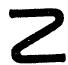
\includegraphics[keepaspectratio]{images/part002_29e6d4b6.jpg}}

Note that the space of all bounded continuous real-valued functions on R, endowed with the topology of uniform convergence, is not of countable type (Exercise 4).

\subsection{THE COMPACT-OPEN TOPOLOGY}

THEOREM 2. Let X be a topological space, Y a uniform space. For each compact subset K of X and each open subset U of Y, let \(\mathbf{T}(\mathbf{K},\mathbf{U})\) denote the set of all continuous mappings \(u:X\to Y\) such that \(u(\mathbf{K})\subset U\) . Then the sets \(\mathbf{T}(\mathbf{K},\mathbf{U})\) generate the topology of compact convergence on \(\mathcal{C}(\mathbf{X};\mathbf{Y})\) .

Let \(Y'\) be the Hausdorff uniform space associated with \(Y\) (Chapter II, § 3, no. 8) and let \(i: Y \to Y'\) be the canonical mapping of \(Y\) onto \(Y'\) . The topology of compact convergence is the coarsest topology for which the mappings \(u \to (i \circ u)|K\) of \(\mathcal{C}(X; Y)\) into \(\mathcal{C}_u(K; Y')\) are continuous, as \(K\) runs through the set of all compact subsets of \(X\) (§ 1, no. 4, Proposition 4). Hence we obtain a subbase of the topology of \(\mathcal{C}_c(X; Y)\) by taking a subbase of the topology of \(\mathcal{C}_c(K; Y')\) for each compact subset \(K\) of \(X\) and then taking the union {[}in \(\mathfrak{P}(\mathcal{C}(X; Y))\) {]} of the inverse images of these subbases in \(\mathcal{C}(X, Y)\) . On the other hand, every open subset of \(Y\) is of the form \(\overline{i}^1(U')\) , where \(U'\) is open in \(Y'\) (Chapter II, § 3, no. 7, Proposition 12); hence, for each compact subset \(K' \supset K\) , \(T(K, \overline{i}^1(U'))\) is the inverse image of \(T(K, U')\) under the mapping

\[
\mathcal {C} (\mathbf {X}; \mathbf {Y}) \rightarrow \mathcal {C} _ {u} (\mathbf {K} ^ {\prime}; \mathbf {Y} ^ {\prime}).
\]

It thus remains for us to prove the theorem when X is compact and Y is Hausdorff; we shall make these assumptions from now on.

Let us first show that \(T(\mathbf{K}, \mathbf{U})\) is open in \(\mathcal{C}_c(\mathbf{X}; \mathbf{Y})\) . Let \(u_0\) be a point of this set; since \(u_0(\mathbf{K})\) is compact (Chapter I, § 9, no. 4, Theorem 2, Corollary 1) and contained in the open set \(\mathbf{U}\) , there exists a symmetric entourage \(\mathbf{V}\) of \(\mathbf{Y}\) such that \(\mathbf{V}(u_0(\mathbf{K})) \subset \mathbf{U}\) (Chapter II, § 4, no. 3, Proposition 4, Corollary). Let \(\mathbf{W}\) be the neighbourhood of \(u_0\) in \(\mathcal{C}_c(\mathbf{X}; \mathbf{Y})\) consisting of all continuous mappings \(u: \mathbf{X} \to \mathbf{Y}\) such that \((u(x), u_0(x)) \in \mathbf{V}\) for all \(x \in \mathbf{K}\) . For such mappings we clearly have \(u(\mathbf{K}) \subset \mathbf{V}(u_0(\mathbf{K})) \subset \mathbf{U}\) ; hence \(u \in T(\mathbf{K}, \mathbf{U})\) and therefore \(W \subset T(\mathbf{K}, \mathbf{U})\) , which proves our assertion.

Conversely, if W is a neighbourhood of a point \(u_{0} \in \mathcal{C}_{c}(\mathbf{X}; \mathbf{Y})\) , let us show that W contains the intersection of a finite number of neighbourhoods of the form \(T(\mathbf{K}, \mathbf{U})\) . We may suppose that W is the set of all \(u \in \mathcal{C}(\mathbf{X}; \mathbf{Y})\) such that \((u(x), u_{0}(x)) \in \mathbf{V}\) for all \(x \in X\) , V being a given entourage of Y. Since \(u_{0}\) is continuous on X, it is uniformly continuous (Chapter II, § 4, no. 1, Theorem 2). Let \(V_{1}\) be a symmetric entourage of Y, open in \(Y \times Y\) and such that \(V_{1}^{2} \subset V\) . X can be covered by a finite number of compact sets \(K_{i}\) ( \(1 \leqslant i \leqslant n\) ) such that each \(u_{0}(\mathbf{K}_{i})\) is \(V_{1}\) -small ( \(1 \leqslant i \leqslant n\) ). Let \(U_{i}\) be the open set \(V_{1}(u_{0}(\mathbf{K}_{i}))\) , and let \(u: X \to Y\) be a continuous mapping contained in the intersection of the n sets \(T(\mathbf{K}_{i}, \mathbf{U}_{i})\) (which are neighbourhoods of \(u_{0}\) ). Then, for every \(x \in K_{i}\) , \(u(x)\) belongs to \(U_{i}\) and therefore \(u_{0}(x)\) and \(u(x)\) are \(V_{1}^{2}\) -close, hence V-close. Since each \(x \in X\) belongs to some \(K_{i}\) , we have \(u \in W\) and the proof is complete.

This result leads us to make the following definition :

DEFINITION 1. Let X, Y be two topological spaces, not necessarily uniformizable. For each compact subset K of X and each open subset U of Y, let T(K, U) be the set of all \(u \in \mathcal{C}(X; Y)\) such that \(u(K) \subset U\) . The topology on C(X; Y) generated by the sets T(K, U) is called the topology of compact convergence or the compact-open topology; and we denote by \(\mathcal{C}_{c}(X; Y)\) the topological space obtained by endowing C(X; Y) with this topology.

If Y is a uniform space it follows from Theorem 2 that this definition agrees with that given in §1, no. 3.

If H is a subset of \(\mathcal{C}(\mathbf{X};\mathbf{Y})\) we shall say that the topology induced on H by that of \(\mathcal{C}_{c}(\mathbf{X};\mathbf{Y})\) is the compact-open topology on H.

Example. Let I be the interval \([0, 1]\) in R. If Y is any topological space, the space \(\mathcal{C}_{c}(I; Y)\) is called the space of paths in Y. For each \(y \in Y\) , the subspace \(\Omega_{y}(Y)\) of \(\mathcal{C}_{c}(I; Y)\) consisting of paths u such that \(u(0) = u(1) = y\) is called the space of loops (in Y) at the point y.

Remarks. 1) Likewise, the topology induced on \(\mathcal{C}(\mathbf{X};\mathbf{Y})\) by the product topology on \(\mathbf{Y}^{\mathbf{X}} = \mathcal{F}(\mathbf{X};\mathbf{Y})\) is called the topology of pointwise convergence (Y being not necessarily uniformizable); it is generated by sets of the form \(T(\{x\}, \mathbf{U})\) as \(x\) runs through \(\mathbf{X}\) and \(\mathbf{U}\) runs through the set of all open subsets of \(\mathbf{Y}\) , and it is therefore coarser than the compact-open topology. We deduce that, if \(\mathbf{Y}\) is Hausdorff, the space \(\mathcal{C}_s(\mathbf{X}; \mathbf{Y})\) is Hausdorff (Chapter I, § 8, no. 1, Proposition 5, Corollary).

\begin{enumerate}
\def\labelenumi{\arabic{enumi})}
\setcounter{enumi}{1}
\tightlist
\item
  Let \(\mathfrak{S}\) be a subbase of the topology of Y, and let \(\mathfrak{R}\) be a set of compact subsets of X with the following property:
\end{enumerate}

\begin{enumerate}
\def\labelenumi{(\Alph{enumi})}
\setcounter{enumi}{17}
\tightlist
\item
  If \(\mathbf{L}\) is any compact subset of \(\mathbf{X}\) and \(\mathbf{V}\) is any neighbourhood of \(\mathbf{L}\) , there exists a finite number of sets \(\mathbf{K}_i \in \mathfrak{R}\) such that \(\mathbf{L} \subset \bigcup_{i} \mathbf{K}_i \subset \mathbf{V}\) .
\end{enumerate}

Then the sets \(T(\mathbf{K}, \mathbf{U})\) , where \(\mathbf{K} \in \mathfrak{R}\) and \(\mathbf{U} \in \mathfrak{S}\) , form a subbase for the compact-open topology on \(\mathcal{C}(\mathbf{X}; \mathbf{Y})\) . To prove this, we have to show that if \(\mathbf{L}\) is any compact subset of \(\mathbf{X}\) and \(\mathbf{V}\) any open subset of \(\mathbf{Y}\) , and if \(u \in T(\mathbf{L}, \mathbf{V})\) , then there exists a finite number of pairs \((\mathbf{K}_i, \mathbf{U}_i)\) such that \(\mathbf{K}_i \in \mathfrak{R}\) , \(\mathbf{U}_i \in \mathfrak{S}\) and \(u \in \bigcap_{i} T(\mathbf{K}_i, \mathbf{U}_i) \subset T(\mathbf{L}, \mathbf{V})\) . Note first that for every finite sequence \((s_k)\) of sets of \(\mathfrak{S}\) and every compact subset \(\mathbf{M}\) of \(\mathbf{X}\) , we have \(T\left(\mathbf{M}, \bigcap_k \mathbf{S}_k\right) = \bigcap_k T(\mathbf{M}, \mathbf{S}_k)\) by definition. We may therefore first of all replace \(\mathfrak{S}\) by the set of finite intersections of sets of \(\mathfrak{S}\) , i.e.~we may suppose that \(\mathfrak{S}\) is a base of the topology of \(\mathbf{Y}\) . By hypothesis, \(u(\mathbf{L})\) is quasi-compact and contained in \(\mathbf{V}\) , hence there exists a finite number of sets \(\mathbf{U}_i \in \mathfrak{S}\) contained in \(\mathbf{V}\) which cover \(u(\mathbf{L})\) . The sets \(\overline{u}^1(\mathbf{U}_i)\) are open in \(\mathbf{X}\) and cover \(\mathbf{L}\) . For each \(x \in \mathbf{L}\) there is therefore a compact neighbourhood \(N_x\) of \(x\) in \(\mathbf{L}\) , contained in some one of the \(\overline{u}^1(\mathbf{U}_i)\) . We can cover \(\mathbf{L}\) with a finite number of these sets \(N_{x_j} = L_j\) ; for each \(j\) , let us denote by \(i(j)\) one of the indices \(i\) such that \(L_j \subset \overline{u}^1(\mathbf{U}_i)\) . This being so, for each index \(j\) there exists {[}by (R){]} a finite number of sets \(K_{jk} \subset \overline{u}^1(\mathbf{U}_{i(j)})\) , belonging to \(\mathfrak{R}\) , which cover \(L_j\) . For each \(v \in \bigcap_{j,k} T(\mathrm{K}_{jk}, \mathrm{U}_{i(j)})\) we have \(\bigcup_{k} v(\mathrm{K}_{jk}) \subset U_{i(j)}\) and therefore \(v(\mathrm{L}_j) \subset U_{i(j)}\) , and \(v(\mathrm{L}) = \bigcup_{j} v(\mathrm{L}_j) \subset \bigcup_{j} U_{i(j)} \subset V\) ; thus our assertion is proved.

THEOREM 3. Let X, Y, Z be three topological spaces and let f be a mapping of X × Y into Z. If f is continuous then \(f: x \to f(x, .)\) is a continuous mapping of X into \(\mathcal{C}_{c}(Y; Z)\) . The converse is true if Y is locally compact.

Suppose that \(f\) is continuous. To show that \(\tilde{f}\) is continuous we have to prove that, for each compact subset \(K\) of \(Y\) and each open subset \(U\) of \(Z\) , the inverse image \(V\) of \(T(K, U)\) under \(\tilde{f}\) is open in \(X\) . Let \(x_0 \in V\) ; for each \(y \in K\) , we have \(f(x_0, y) \in U\) , and since \(f\) is continuous there is a neighbourhood \(V_y\) of \(x_0\) in \(X\) and a neighbourhood \(W_y\) of \(y\) in \(Y\) such that \(f(V_y \times W_y) \subset U\) . Since \(K\) is compact, there exists a finite number of points \(y_{i} \in K\) such that the sets \(W_{y_{i}}(1 \leqslant i \leqslant n)\) cover K. Let \(V'\) be the intersection of the neighbourhoods \(V_{y_{i}}\) of \(x_{0}\) , which is a neighbourhood of \(x_{0}\) ; if \(x \in V'\) and \(y \in K\) , we have \(f(x, y) \in U\) , since y is contained in some one of the \(W_{y_{i}}\) and x is contained in each \(V_{y_{i}}\) ; hence \(V' \subset V\) , and therefore V is a neighbourhood of each of its points and consequently is open in X.

Conversely, suppose that \(\tilde{f}\) is continuous and that Y is locally compact, and let us show that \(f\) is continuous. Let \(x_0 \in \mathbf{X}\) , let \(y_0 \in \mathbf{Y}\) and let U be an open neighbourhood of \(f(x_0, y_0)\) in Z; we shall show that there is a neighbourhood V of \(x_0\) in X and a neighbourhood W of \(y_0\) in Y such that \(f(\mathbf{V} \times \mathbf{W}) \subset \mathbf{U}\) . Since \(y \to f(x_0, y)\) is continuous, there is a compact neighbourhood W of \(y_0\) such that \(f(\{x_0\} \times \mathbf{W}) \subset \mathbf{U}\) . On the other hand, since \(\tilde{f}\) is continuous, the set V of \(x \in \mathbf{X}\) such that \(f(x, .) \in T(\mathbf{W}, \mathbf{U})\) {[}i.e.~such that \(f(x, y) \in \mathbf{U}\) for all \(y \in \mathbf{W}]\) is an open subset of X and therefore a neighbourhood of \(x_0\) ; and we have \(f(\mathbf{V} \times \mathbf{W}) \subset \mathbf{U}\) .

Q.E.D.

COROLLARY I. Let X be a locally compact space, Y a topological space, H a subset of C (X; Y). Then the compact-open topology on H is the coarsest for which the mapping \((u, x) \to u(x)\) of \(H \times X\) into Y is continuous.

For, by Theorem 3, this mapping is continuous if and only if the canonical injection \(\mathbf{H} \to \mathcal{C}_c(\mathbf{X}; \mathbf{Y})\) is continuous.

Remark. 3) Let X be a locally compact space and Y a Hausdorff topological space. If \(\mathcal{G}\) is a topology on a subset H of \(\mathcal{C}(\mathbf{X};\mathbf{Y})\) such that the mapping \((u,x)\to u(x)\) is continuous on \(\mathrm{H}\times \mathrm{X}\) and if also H is compact with respect to \(\mathcal{G}\) , then \(\mathcal{G}\) is the compact-open topology. For it is finer than the latter by Corollary 1, and since the compact-open topology is Hausdorff, the two topologies are identical. Note that if in addition Y is completely regular, then H is equicontinuous with respect to every uniformity compatible with the topology of Y (§2, no. 5, Theorem 2, Corollary 3), and for every compact subset K of X the set

\[
\mathrm{H} (\mathrm{K}) = \bigcup_ {x \in \mathrm{K}} \mathrm{H} (x)
\]

is compact, since it is the image of \(\mathbf{H} \times \mathbf{K}\) under the continuous mapping \((u, x) \to u(x)\) .

COROLLARY 2. Let X, Y, Z be three topological spaces such that X is Hausdorff and Y is locally compact. Then the restriction to \(\mathcal{C}(\mathbf{X} \times \mathbf{Y}; \mathbf{Z})\) of the canonical bijection \(\mathcal{F}(\mathbf{X} \times \mathbf{Y}; \mathbf{Z}) \to \mathcal{F}(\mathbf{X}; \mathcal{F}(\mathbf{Y}; \mathbf{Z}))\) (Set Theory, R, §4, no. 14) is a homeomorphism of \(\mathcal{C}_c(\mathbf{X} \times \mathbf{Y}; \mathbf{Z})\) onto \(\mathcal{C}_c(\mathbf{X}; \mathcal{C}_c(\mathbf{Y}; \mathbf{Z}))\) .

This restriction is certainly a bijection

\[
\rho : \mathcal {C} (\mathrm{X} \times \mathrm{Y}; \mathrm{Z}) \rightarrow \mathcal {C} (\mathrm{X}; \mathcal {C} _ {c} (\mathrm{Y}; \mathrm{Z}))
\]

by Theorem 3; it remains therefore to be shown that the compact-open topology on \(\mathcal{C}(\mathbf{X}\times\mathbf{Y};\mathbf{Z})\) is the inverse image under \(\rho\) of the compact-open topology on \(\mathcal{C}(\mathbf{X};\mathcal{C}_{c}(\mathbf{Y};\mathbf{Z}))\) . Since the sets \(T(\mathbf{K},\mathbf{U})\) , where \(\mathbf{K}\) is a compact subset of \(\mathbf{Y}\) and \(\mathbf{U}\) is an open subset of \(\mathbf{Z}\) , form a subbase of the topology of \(\mathcal{C}_{c}(\mathbf{Y};\mathbf{Z})\) , it follows from Remark 2 that the topology of \(\mathcal{C}_{c}(\mathbf{X};\mathcal{C}_{c}(\mathbf{Y};\mathbf{Z}))\) is generated by the sets of the form \(T(J,T(\mathbf{K},\mathbf{U}))\) , where \(\mathbf{K}\) and \(\mathbf{U}\) are as above and \(J\) is a compact subset of \(\mathbf{X}\) . Now the image of \(T(J,T(\mathbf{K},\mathbf{U}))\) under \(\rho\) is precisely \(T(J\times K,\mathbf{U})\) , and is therefore an open set; so we have shown that \(\rho\) is continuous. To prove that \(\rho\) is a homeomorphism, we note first that the sets of the form \(J\times K\) in \(\mathbf{X}\times\mathbf{Y}\) (where \(J\) is a compact subset of \(\mathbf{X}\) , and \(\mathbf{K}\) is a compact subset of \(\mathbf{Y}\) ) satisfy the condition (R) of Remark 2: for if \(\mathbf{L}\) is a compact subset of \(\mathbf{X}\times\mathbf{Y}\) and \(\mathbf{V}\) is a neighbourhood of \(\mathbf{L}\) in \(\mathbf{X}\times\mathbf{Y}\) , the projections \(M=pr_{1}(L)\) , \(N=pr_{2}(L)\) are compact, since \(\mathbf{X}\) and \(\mathbf{Y}\) are Hausdorff and \(V\cap(M\times N)\) is a neighbourhood of \(\mathbf{L}\) in the compact space \(M\times N\) , so that every point of \(\mathbf{L}\) has a neighbourhood in \(M\times N\) of the form \(J\times K\subset V\) , where \(J\subset M\) and \(K\subset N\) are compact; since \(\mathbf{L}\) can be covered by a finite number of these neighbourhoods, the assertion is proved. Therefore sets of the form \(T(J\times K;\mathbf{U})\) , where \(J\) is a compact subset of \(\mathbf{X},\mathbf{K}\) a compact subset of \(\mathbf{Y}\) and \(\mathbf{U}\) an open subset of \(\mathbf{Z}\) , generate the topology of \(\mathcal{C}_{c}(\mathbf{X}\times\mathbf{Y};\mathbf{Z})\) . But we have already seen that the image of \(T(J\times K,\mathbf{U})\) under \(\rho\) is the open set \(T(J,T(K,\mathbf{U}))\) in \(\mathcal{C}_{c}(\mathbf{X};\mathcal{C}_{c}(\mathbf{Y};\mathbf{Z}))\) ; hence \(\rho\) is a homeomorphism.

Note that if in addition Z is assumed to be uniformizable, Corollary 2 is a trivial consequence of § 1, no. 4, Proposition 2.

PROPOSITION 9. Let X, Y, Z be three topological spaces, Y being locally compact. Then the mapping \((u, v) \to v \circ u\) of \(\mathcal{C}_c(X; Y) \times \mathcal{C}_c(Y; Z)\) into \(\mathcal{C}_c(X; Z)\) is continuous.

We have to show that, for every compact subset K of X and every open subset U of Z, the set R of pairs \((u, v)\) such that \(v(u(\mathbf{K})) \subset \mathbf{U}\) is open in \(\mathcal{C}_{c}(\mathbf{X}; \mathbf{Y}) \times \mathcal{C}_{c}(\mathbf{Y}; \mathbf{Z})\) . Let \((u_{0}, v_{0}) \in R\) ; then \(u_{0}(\mathbf{K})\) is a compact subset of the locally compact space Y, contained in the open set \(\overline{v}_{0}^{1}(\mathbf{U})\) , and hence there is a compact neighbourhood L of \(u_{0}(\mathbf{K})\) contained in \(\overline{v}_{0}^{1}(\mathbf{U})\) (Chapter I, § 9, no. 7, Proposition 10). The set V of all \(u \in C_{c}(\mathbf{X}; \mathbf{Y})\) such that \(u(\mathbf{K}) \subset \mathring{\mathbf{L}}\) is a neighbourhood of \(u_{0}\) , and the set W of all \(v \in C_{c}(\mathbf{Y}; \mathbf{Z})\) such that \(v(\mathbf{L}) \subset \mathbf{U}\) is a neighbourhood of \(v_{0}\) ; furthermore, the relation \((u, v) \in \mathbf{V} \times \mathbf{W}\) implies \(v(u(\mathbf{K})) \subset \mathbf{U}\) . Hence the result.

\subsection{TOPOLOGIES ON GROUPS OF HOMEOMORPHISMS}

PROPOSITION 10. Let X be a uniform space and let H be an equicontinuous set of homeomorphisms of X onto itself. If H and \(H^{-1}\) are endowed with the topology of pointwise convergence in X, then the mapping \(u \rightarrow u^{-1}\) of \(H^{-1}\) onto H is continuous.

It is enough to show that, for each \(x_0 \in \mathbf{X}\) , the mapping \(u \to u^{-1}(x_0)\) of \(\mathbf{H}^{-1}\) into \(\mathbf{X}\) is continuous at every point \(u_0 \in \mathbf{H}^{-1}\) . Let \(\mathbf{V}\) be a symmetric entourage of \(\mathbf{X}\) , and let \(y_0 = u_0^{-1}(x_0)\) . By hypothesis there is a symmetric entourage \(\mathbf{U}\) of \(\mathbf{X}\) such that the relation \((x, x_0) \in \mathbf{U}\) implies \((u^{-1}(x), u^{-1}(x_0)) \in \mathbf{V}\) for all \(u \in \mathbf{H}^{-1}\) . Take an element \(u \in \mathbf{H}^{-1}\) which is \(W(\{y_0\}, \mathbf{U})\) -close to \(u_0\) ; then we have \((u(y_0), u_0(y_0)) \in \mathbf{U}\) , i.e.~\((u(y_0), x_0) \in \mathbf{U}\) . It follows that \((y_0, u^{-1}(x_0)) \in \mathbf{V}\) , i.e.~\((u_0^{-1}(x_0), u^{-1}(x_0)) \in \mathbf{V}\) ; this completes the proof.

COROLLARY. Let X be a uniform space and let H be an equicontinuous group of homeomorphisms of X onto itself. Then the topology of pointwise convergence in X is compatible with the group structure of H.

This is a consequence of Proposition 10, together with § 2, no. 1, Proposition 1, Corollary 5.

PROPOSITION II. Let X be a compact space and let \(\Gamma\) be the group of all homeomorphisms of X onto itself. Then the topology of uniform convergence in X is compatible with the group structure of \(\Gamma\) .

We know already (no. 4, Proposition 9) that the mapping \((u, v) \to v \circ u\) of \(\Gamma \times \Gamma\) into \(\Gamma\) is continuous with respect to this topology; thus we have to show that \(u \to u^{-1}\) is continuous at every point \(u_0\) of \(\Gamma\) . Since \(u_0^{-1}\) is uniformly continuous on \(\mathbf{X}\) , given any symmetric entourage \(\mathbf{V}\) of \(\mathbf{X}\) there exists an entourage \(\mathbf{W}\) of \(\mathbf{X}\) such that the relation \((x, x') \in \mathbf{W}\) implies \((u_0^{-1}(x), u_0^{-1}(x')) \in \mathbf{V}\) . Hence, if \(u \in \Gamma\) is such that \((u_0(x), u(x)) \in \mathbf{W}\) for all \(x \in \mathbf{X}\) , it follows that \((x, u_0^{-1}(u(x))) \in \mathbf{V}\) for all \(x \in \mathbf{X}\) , and therefore (as \(u\) is bijective) \((u^{-1}(x), u_0^{-1}(x)) \in \mathbf{V}\) for all \(x \in \mathbf{X}\) . This completes the proof.

\pandocbounded{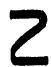
\includegraphics[keepaspectratio]{images/part002_d26bd6ea.jpg}}

Now let X be a locally compact space and let \(\Gamma\) be the group of all homeomorphisms of X onto itself. The topology of compact convergence in X is not necessarily compatible with the group structure of \(\Gamma\) (Exercise 17). Let \(X'\) denote the compact space obtained by adjoining a point at infinity \(\omega\) to X. Every homeomorphism u of X onto itself extends uniquely to a homeomorphism \(u'\) of \(X'\) onto itself such that \(u'(\omega) = \omega\) (Chapter I, § 10, no. 3, Corollary to Proposition 7), so that \(\Gamma\) can be identified with the subgroup of the group \(\Gamma'\) of all homeomorphisms of \(X'\) onto itself, consisting of all homeomorphisms which leave \(\omega\) fixed. The topology induced on \(\Gamma\) by that of \(C_u(X'; X')\) is therefore compatible with the group structure of \(\Gamma\) (Proposition 11), and \(\Gamma\) is closed in \(\Gamma'\) {[}with respect to the topology induced by that of \(\mathcal{C}_u(\mathbf{X}';\mathbf{X}')\) {]} because it is defined by the equation \(u(\omega)=\omega\) ( \(\S\) 1, no. 2, Remark 6). We denote by \(\mathcal{C}_{\beta}\) the group topology thus defined on \(\Gamma\) ; it is finer than the topology of compact convergence and can also (by virtue of \(\S\) 1, no. 6, Proposition 6) be defined as the topology of uniform convergence on \(\mathbf{X}\) , when \(\mathbf{X}\) is endowed with the uniformity induced by the unique uniformity of \(\mathbf{X}'\) .

The topology \(\mathcal{C}_{\beta}\) can be characterized as follows:

PROPOSITION 12. On the group \(\Gamma\) of all homeomorphisms of a locally compact space \(\mathbf{X}\) , the topology \(\mathcal{C}_{\beta}\) is the coarsest for which the mappings \(u \to u\) and \(u \to u^{-1}\) of \(\Gamma\) into \(\mathcal{C}_c(\mathbf{X}; \mathbf{X})\) are continuous.

Let us denote the latter topology for the moment by \(\mathcal{C}'\) . Since \(u \to u^{-1}\) is continuous with respect to \(\mathcal{C}_{\beta}\) and since \(\mathcal{C}_{\beta}\) is finer than the topology of compact convergence, it is clear that \(\mathcal{C}_{\beta}\) is finer than \(\mathcal{C}'\) . To prove the converse, endow \(\mathbf{X}'\) with its unique uniformity; let \(u_0 \in \Gamma\) and let \(\mathbf{V}\) be an entourage of \(\mathbf{X}'\) ; then we have to prove that there is a compact subset \(\mathbf{K}\) of \(\mathbf{X}\) and a symmetric entourage \(\mathbf{W}\) of \(\mathbf{X}'\) such that the relations

\[
u \in \Gamma , (u _ {0} (x), u (x)) \in \mathrm{W} \text {   and   } (u _ {0} ^ {- 1} (x), u ^ {- 1} (x)) \in \mathrm{W} \text {   for   all   } x \in \mathrm{K}
\]

imply

\[
(u _ {0} (x), u (x)) \in \mathbf {V} \text {   for   all   } x \in \mathbf {X}.
\]

Let \(V_1\) be a symmetric open entourage of \(X'\) such that \(\dot{V}_1 \subset V\) ; then \(K_1 = X' - V_1(\omega)\) is a compact subset of \(X\) . Choose a symmetric open entourage \(W\) of \(X'\) such that \(W \subset V\) and \(W(\omega) \cap W(u_0^{-1}(K_1)) = \emptyset\) ; this is possible by Proposition 4 of Chapter II, § 4, no. 3. Let \(K_2 = X' - W(\omega)\) , which is a compact subset of \(X\) . We shall see that \(W\) and the compact set \(K = K_1 \cup K_2\) do what is required. Since \(W \subset V\) , it is enough to show that the relation

\[
\left(u _ {0} ^ {- 1} (x), u ^ {- 1} (x)\right) \in \mathrm{W} \quad \text { for   all } \quad x \in \mathrm{K} _ {1} \quad (u \in \Gamma)
\]

implies that

\[
(u (y), \omega) \in \mathrm{V} _ {1} \quad \text { for   all } \quad y \in \mathrm{W} (\omega);
\]

for we shall then also have \((u_0(y),\omega)\in \mathbf{V}_1\) and thence

\[
(u _ {0} (y), u (y)) \in \mathring {\mathrm{V}} _ {1} ^ {2} \subset \mathrm{V}
\]

for all \(y \in W(\omega) = X' - K_2\) . Now if we had \(y \in W(\omega)\) and

\[
u (y) \in \mathrm{X} ^ {\prime} - \mathrm{V} _ {1} (\omega) = \mathrm{K} _ {1},
\]

it would follow that \(y \in u^{-1}(\mathbf{K}_1) \subset W(u_0^{-1}(\mathbf{K}_1))\) , contrary to the choice of \(W\) ; the proof is therefore complete.

In general the group \(\Gamma\) , endowed with \(\mathfrak{G}_{\beta}\) , is not locally compact; but we have the following criterion:

THEOREM 4. Let G be a subgroup of the group \(\Gamma\) of all homeomorphisms of a locally compact space X. Suppose that, in the space \(\mathcal{C}_{\mathfrak{c}}(\mathbf{X};\mathbf{X})\) , there is a neighbourhood V of the identity mapping \(e\) such that \(\mathbf{V}\cap \mathbf{G} = \mathbf{H}\) is symmetric in G and relatively compact in \(\mathcal{C}_{\mathfrak{c}}(\mathbf{X};\mathbf{X})\) . Then the closure \(\overline{\mathbf{G}}\) of G in \(\Gamma\) with respect to the topology \(\mathcal{T}_{\beta}\) is a locally compact group with respect to the topology induced by \(\mathcal{T}_{\beta}\) ; this topology induced on \(\overline{\mathbf{G}}\) is the same as the topology of compact convergence, and the closure \(\overline{\mathbf{H}}\) of H in \(\mathcal{C}_{\mathfrak{c}}(\mathbf{X};\mathbf{X})\) is a neighbourhood of \(e\) in \(\overline{\mathbf{G}}\) with respect to this topology.

Let us show first that \(\overline{\mathbf{H}}\) is contained in \(\Gamma\) and that the topology induced on \(\overline{\mathbf{H}}\) by \(\mathfrak{C}_{\beta}\) is the same as the topology of compact convergence. Let \(u_0 \in \overline{\mathbf{H}}\) ; \(u_0\) is therefore the limit, in \(\mathcal{C}_c(\mathbf{X}; \mathbf{X})\) , of an ultrafilter \(\Phi\) on \(\mathbf{H}\) . Since \(\Phi^{-1}\) (the image of \(\Phi\) under \(u \to u^{-1}\) ) is an ultrafilter base on \(\mathbf{H} \subset \overline{\mathbf{H}}\) , it converges in the compact subspace \(\overline{\mathbf{H}}\) of \(\mathcal{C}_c(\mathbf{X}; \mathbf{X})\) to an element \(v_0\) . The mapping \((u, v) \to uv\) converges to \(u_0 v_0\) with respect to \(\Phi \times \Phi^{-1}\) (no. 4, Proposition 9); a fortiori, \(u \to uu^{-1} = e\) converges to \(u_0 v_0\) with respect to \(\Phi\) , hence \(u_0 v_0 = e\) since \(\mathcal{C}_c(\mathbf{X}; \mathbf{X})\) is Hausdorff. Similarly \(v_0 u_0 = e\) ; hence \(u_0\) is a homeomorphism of \(\mathbf{X}\) , i.e., \(u_0 \in \Gamma\) . Thus \(\overline{\mathbf{H}}\) is contained in \(\Gamma\) . Moreover, this argument shows that \(\overline{\mathbf{H}}^{-1} = \overline{\mathbf{H}}\) and that, for every ultrafilter \(\Phi\) on \(\overline{\mathbf{H}}\) which converges to \(u_0\) , \(\Phi^{-1}\) converges in \(\mathcal{C}_c(\mathbf{X}; \mathbf{X})\) to \(u_0^{-1}\) ; hence the mapping \(u \to u^{-1}\) of \(\overline{\mathbf{H}}\) into \(\mathcal{C}_c(\mathbf{X}; \mathbf{X})\) is continuous when \(\overline{\mathbf{H}}\) carries the topology of compact convergence (Chapter I, § 7, no. 4, Proposition 9, Corollary 1). Proposition 12 then shows that, on \(\overline{\mathbf{H}}\) , the topology of compact convergence is the same as the topology induced by \(\mathfrak{C}_{\beta}\) .

Furthermore, since the topology \(\mathcal{C}_{\beta}\) on \(\Gamma\) is finer than the topology of compact convergence, \(\overline{\mathbf{H}}\) is also the closure of \(\mathbf{H}\) with respect to \(\mathcal{C}_{\beta}\) . But \(\mathbf{H}\) is a neighbourhood of \(e\) in \(\mathbf{G}\) with respect to the topology of compact convergence, and a fortiori with respect to the topology induced by \(\mathcal{C}_{\beta}\) ; it follows (Chapter I, § 3, no. 1, Proposition 2) that \(\overline{\mathbf{H}}\) is a neighbourhood of \(e\) in \(\overline{\mathbf{G}}\) with respect to the topology induced by \(\mathcal{C}_{\beta}\) , and hence \(\overline{\mathbf{G}}\) is locally compact in this topology. If \(\mathbf{W}\) is the interior of \(\mathbf{V}\) with respect to the topology of compact convergence, then \(\mathbf{W} \cap \Gamma\) is open in \(\mathcal{C}_{\beta}\) , hence \(\mathbf{W} \cap \overline{\mathbf{G}}\) is contained in the closure of \(\mathbf{H} = \mathbf{V} \cap \mathbf{G}\) with respect to \(\mathcal{C}_{\beta}\) (Chapter I, § 1, no. 6, Proposition 5); this shows that \(\overline{\mathbf{H}}\) is also a neighbourhood of \(e\) in \(\overline{\mathbf{G}}\) with respect to the topology of compact convergence. Finally, for each \(u_{0} \in \Gamma\) , the bijections \(v \to u_{0} \circ v\) and \(v \to u_{0}^{-1} \circ v\) of \(\mathcal{C}_{c}(\mathbf{X}; \mathbf{X})\) onto itself are continuous (no. 4, Proposition 9), and hence, if \(u_{0} \in \overline{G}\) , \(u_{0}\overline{H}\) is a neighbourhood of \(u_{0}\) in \(\overline{G}\) with respect to the topology of compact convergence. This completes the proof.

COROLLARY. Let G be a group of homeomorphisms of a locally compact space X. If the closure \(\overline{G}\) of G in \(\mathcal{C}_{c}(X; X)\) is compact, then \(\overline{G}\) is a group of homeomorphisms of X, and the topology of compact convergence is compatible with the group structure of \(\overline{G}\) , which is therefore a compact topological group.

\pandocbounded{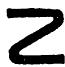
\includegraphics[keepaspectratio]{images/part002_e2b18e11.jpg}}

A group of homeomorphisms of a locally compact space X which is locally compact but not compact with respect to the topology of compact convergence is locally closed in \(\mathcal{C}_{c}(\mathbf{X};\mathbf{X})\) by virtue of Chapter I, § 9, no. 7, Proposition 12, but is not necessarily closed.

For example, in the ring \(\mathcal{L}(\mathbf{R}^{n})\) of endomorphisms of \(\mathbf{R}^{n}\) , identified with the ring \(\mathbf{M}_{n}(\mathbf{R})\) of square \(n \times n\) matrices over \(\mathbf{R}\) and endowed with the topology of compact convergence, the group \(\mathbf{GL}(n, \mathbf{R})\) , identified with the group of non-singular matrices, is locally compact but dense (Chapter VI, § 1, no. 6, Proposition 6).

\section{APPROXIMATION OF CONTINUOUS REAL-VALUED FUNCTIONS}
